%
%	Documento de plan de proyecto
%

\documentclass[11pt, a4paper, twoside, titlepage]{article}
\usepackage[utf8x]{inputenc}
\usepackage[T1]{fontenc}
\usepackage[spanish]{babel}
\usepackage{lmodern}
\usepackage{anysize}
\usepackage[none]{hyphenat}
\usepackage{multicol}
\usepackage{amsmath}
\usepackage[colorlinks, linkcolor=red]{hyperref}
\usepackage[doc=planproyecto]{isdiedral}
\usepackage{lscape}
\usepackage{float}

% Nombre del documento (para futuras referencias)
\newcommand*{\doctitle}{Plan de proyecto}
\newcommand*{\docversion}{2.0}

%%% Configuraciones %%%
\marginsize{2.5cm}{2cm}{2cm}{2cm}

% Usa como familia tipográfica por defecto "Sans"
\renewcommand{\familydefault}{\sfdefault}

% Establece la profundidad hasta la cual se numeran los elementos de sección
\setcounter{secnumdepth}{4}

% Configuración de los encabezados
\encabezadodiedral{\doctitle{} \docversion}
\pagestyle{fancy}
\renewcommand*{\thepage}{\sffamily \roman{page}}

% Modelo copiado de los apuntes del tema 5 pág 69 (a lo Pressman)

\title{\doctitle\\\textsl{Airline Common Environment}}
\author{Grupo Diedral}

% Metadatos del pdf
\hypersetup{
pdfinfo={
	Author={Grupo Diedral},
	Title={\doctitle{} \docversion},
	Subject={Airline Common Environment},
	Keywords={Plan de proyecto;Airline Common Environment;Ingeniería del Software}
}
}

\begin{document}
	% Tabla de cambios
	\begin{tablacambios}
		2.0 & 28 de febrero de 2013 & CAF, NAH, SBC, JCP, RRC & Segunda entrega
	\end{tablacambios}

	% Fija la cita inicial
	\fijacitainicial{Difícil de ver el futuro es}{Maestro Yoda, Star Wars: La Venganza de los Sith}

	% Portada
	\portadaace{\doctitle}{\docversion}
	
	\tableofcontents
	\newpage

	\section{Introducción}
	\iniciarnumeraciondiedral
		\subsection{Propósito del plan}
			Este documento pretende servir de guía para el proceso de desarrollo del \software \textit{Airline Common Environment}. Los principales puntos de este plan incluyen un estudio de los riesgos a los que está sometido nuestro proyecto, además de la estimación de coste y duración del mismo, seguida de la correspondiente planificación. Versiones futuras del documento incorporarán el análisis sobre garantía de calidad y la gestión de configuración, que ya están parcialmente desarrolladas.\\

			Este documento no es un documento estático y será paulatinamente completado y refinado durante todo el proyecto.
		
		\subsection{Ámbito del proyecto y objetivos}
			\subsubsection{Declaración del ámbito}
			El cliente del proyecto es una compañía aérea ya asentada en el sector, por lo que el software está destinado a la sustitución del sistema actual de la compañía que se ha quedado obsoleto y tiene un dificil mantenimiento y escalabilidad, por ello se requerirá de una fase previa a la transición de simulación y pruebas para conseguir una transición segura y sin provocar una parada en la actividad normal de la empresa.
			En cuanto al equipo de desarrollo, se enfrenta por primera vez a un proyecto de esta embergadura por lo que esta especificación y el resto de documentación será susceptible de cambios a lo largo de todo el desarrollo.
			En el marco competitivo, es cierto que existen alternativas generales en el mercado, pero nuestro proyecto pretende ser una solución a medida, viendose ello potenciado por la continua presencia y participación del cliente a lo largo del proyecto.

			\subsubsection{Funciones principales}
			Las funciones principales de la aplicación interna son la consulta de horarios y nóminas para todos los empleados de la compañía, así como otras funciones específicas según el empleo que realicen dentro de la empresa como consultar, añadir o editar distintos datos de empleados, inventario o información de la empresa, y otras funciones concretas relativas al empleo como puede ser realizar un mantenimiento o registrar un nuevo empleado. \\

			La aplicación externa permitirá al cliente la compra de billetes de vuelo, pudiendo realizar el pago por diversos métodos. Además, permitirá la consulta de los vuelos ofertados así como ver información de las diversas ofertas y presentar sugerencias.
			
			\subsubsection{Aspectos de rendimiento}
			El sistema interno podrá reconocer hasta 4.000 terminales. Deberá soportar hasta 1.000 usuarios conectados de forma simultánea a los servicios del software de gestión interna de la aplicación que requieran una conexión latente, e incluso se podrán soportar los 2.000 usuarios si se tratan de conexiones de corta duración.  En cuanto al servidor web, admitirá hasta 6.000 conexiones simultáneas para el contenido estático(no necesita interacción con el servidor de la base de datos). \\

			El 90 por ciento de las transacciones deberán realizarse en menos de un minuto. La base de datos es un elemento crítico en el rendimiento del sistema y deberá ofrecer una alta disponibilidad, puesto que se prevén realizar miles de interacciones al día.

			\subsubsection{Restricciones y técnicas de gestión}
			El rendimiento y las restricciones del sistema están íntimamente relacionadas. La aplicación de gestión interna deberá estar disponible tanto en Linux como en Microsoft Windows XP, Vista y 7; y se podrán considerar Apple Mac OS X 10.X y Solaris en futuras versiones.  \\

			La aplicación se diseñará de acuerdo con los estándares reconocidos, para facilitar así su reutilización y adaptación. Además, el programa debe proporcionar mecanismos para la realización de controles de funcionamiento y auditorías. También hay que asegurar que el sistema quede protegido frente a intentos de accesos externos, respetando en todo momento las regulaciones de protección de datos de carácter personal.

		\subsection{Modelo de proceso}
		El desarrollo de nuestro proyecto estará basado en el modelo conocido como Proceso Unificado también conocido como RUP(Rational Unified Process). Éste modelo fue inicialmente descrito en 1999 por los desarrolladores del lenguaje UML, Ivar Jacobson, Grady Booch y James Rumbaugh y se caracteriza principalmente por estar dirigido por los casos de usos, centrarse en la arquitectura y ser iterativo incremental. En él podemos diferenciar cuatro fases. En la fase de inicio se desarrolla una descripción del producto final, en la fase de elaboración se especifican los casos de uso y se diseña la arquitectura del sistema, en la fase de construcción se crea el producto y por último en la fase de transición se entrega el producto al cliente.

	\section{Estimaciones del proyecto}
		\subsection{Datos históricos}
		A lo largo del documento de planificación temporal nos hemos apoyado en el plan de proyecto de algunos trabajos de la Universidad Complutense como por ejemplo IronHand, Estubox, sobre todo para la identificación de riesgos, tal y como sugiere la Gestión de Riesgos Boehm. Además, también nos hemos ayudado de \cite{PSMAN} y sobre todo de los Top 10 Risk.
		\subsection{Técnicas de estimación}
		Para estimar el coste de nuestro proyecto software de la manera más precisa y dentro del tiempo disponible para ello, hemos intentado retrasar la estimación lo máximo posible, tomando como referencia algunos datos de otros proyectos similares ya terminados. Concretamente, hemos utilizado las técnicas de descomposición basadas en el problema, según el tamaño del software a desarrollar en puntos de función (PF), ayudándonos de modelos como el COCOMO (COnstructive COst MOdel).
		\subsection{Estimaciones de esfuerzo, coste y duración}
			\subsubsection{Discusión de los factores de ajuste} \label{estimac:factores}
				En este epígrafe se discutirán brevemente los factores de ajuste escogidos para la estimación del proyecto de acuerdo al método de puntos de función y los factores de escala y coste de Cocomo II.

				\begin{enumerate}
					\item \textbf{Comunicación de datos}: (5) más de un front-end, más de un protocolo de comunicación.\\
						El \software desarrollado tiene dos interfaces, una interna de tipo escritorio sobre la
					red corporativa; y otra externa basada en web y de acceso por medio de Internet.

					\item \textbf{Funciones distribuidas}: (4) proceso distribuido y transferencia de datos on-line. Ambas direcciones.\\
						El \software en desarrollo es principalmente un programa que gestiona bases de datos. El proceso de la información estará distribuido entre el servidor y el cliente. Cierta información será procesada por el servidor antes de ser enviada al cliente. Así mismo, el cliente procesará la información que le sea introducida por el usuario antes de hacer la correspondiente petición al servidor.

					\item \textbf{Rendimiento}: (2) Tiempo de respuesta o capacidad de proceso crítico durante horas punta.
No diseño especial para utilización CPU.
	
					\item \textbf{Configuraciones fuertemente utilizadas}: (4) Las restricciones obligan a limitaciones en la
aplicación.
					\item \textbf{Frecuencia de transacciones}: (3) Periodo punta diario.
					\item \textbf{Entradas de datos-online}: (3) 16\% al 23\% de las transacciones son interactivas.
					\item \textbf{Eficiencia del usuario final}: (4) 6 o más, con requisitos de eficiencia que obligan a
minimizar por ej. el número de tecleos o a usar máscaras.\\
						Es requerida la pronta validación de los datos introducidos por el usuario y la elaboración de pantallas personalizables para el acceso a las tareas más frecuentes.
					\item \textbf{Actualización on-line de los ILF}: (4) Actualización de los principales ILF, la protección
contra pérdida de datos es esencial y ha sido especialmente diseñada y programada.\\
						La mayor parte de los ILF de la aplicación se actualizan de forma remota a través del \software clientes, ya sea externo o interno.s
					\item \textbf{Procesos complejos}: (1) Proceso lógico completo.

					\item \textbf{Reusabilidad}: (4) La aplicación se empaquetó y/o documentó para ser fácilmente reusable.
Aplicación adaptada por el usuario a nivel de código fuente.\\
						La aplicación está documentada y organizada para facilitar la reutilización. Pese a que algunas adaptaciones están especificadas para poder realizarse a través de la configuración post-compilación, la mayoría de los cambios se han de realizar sobre el código fuente.
					\item \textbf{Facilidad de instalación}: (2) Requisitos de conversión e instalación definidos por usuario.
No se considera importante el impacto de la conversión.
					\item \textbf{Facilidad de operación}: (2) Se minimiza la necesidad de montaje de cintas y manejo de
papel.
					\item \textbf{Instalación en distintos lugares}: (3) Múltiples lugares con entornos distintos de hw y sw.\\
						Es el caso de la aplicación interna que se instalará en los distintos equipos repartidos por las instalaciones de la compañía aérea.
					\item \textbf{Facilidad de cambios}: (3) Facilidad para realizar consultas/informes simples.	
				\end{enumerate}

				Los valoraciones correspondientes a Cocomo son:
				
				\begin{itemize}

				\item Factores de escala

				\begin{enumerate}
					\item \textbf{Experiencia previa}: baja.
					\item \textbf{Flexibilidad del desarrollo}: baja.
					\item \textbf{Resolución de riesgo/arquitectura}: baja.
					\item \textbf{Cohesión del equipo}: alta.
					\item \textbf{Madurez del proceso}: nominal (Proceso Unificado)
				\end{enumerate}

				\item Factores de coste (previo al diseño)

				\begin{enumerate}
					\item \textbf{Fiabilidad requerida}: alta.
					\item \textbf{Reusabilidad}: alta.
					\item \textbf{Complejidad de producto}: alta.
					\item \textbf{Capacidad del personal}: nominal.
					\item \textbf{Experiencia del personal}: baja.
					\item \textbf{Facilidades}: alta.
					\item \textbf{Calendario restringido}: alta.
				\end{enumerate}

				\end{itemize}

			%% El detalle de las estimaciones está desarrollado en archivos aparte

			\subsubsection{Gestión corriente de la base de datos} \label{estimac:gestioncorriente}
						\begin{enumerate}
			\item \textit{FLI}
			\begin{itemize}
				\item Clientes \\
					1 RET(Personales) \\
					11 DET(Nombre, apellidos, e-mail, NIF, teléfono, dirección(6)) \\
					Complejidad: Baja\\
				\item Empleados \\
					2 RET(Personales, Laborales)
					15 DET(Nombre, apellidos, NIF, e-mail, teléfono, dirección(6), puesto trabajo, permisos, registros, periodo laboral)
					Complejidad: Baja\\
				\item Vuelos\\
					1 RET(General)
					7 DET(Número de vuelo, fecha de salida/llegada, hora de salida, hora de llegada, aeropuerto de origen, aeropuerto destino,
					clase)
					Complejidad: Baja\\
				\item Ofertas\\
					3 RET(Descripción, prestaciones, restricciones)
					6 DET(Titulo, resumen, articulo, precio ofertado, periodo validez, ámbito de validez)
					Complejidad: Baja\\
				\item Nóminas\\
					1 RET(Registro)
					8 DET(Identificador del empleado(5)(nombre, apellidos, NIF, nº SS, departamento), incidencias(3)(horas extras,
					sustituciones, huelgas))
					Complejidad: Baja\\
				\item Inventario\\
					1 RET(Descriptivos)
					7 DET(Nombre articulo, número, cantidad, precio de compra, departamento, proveedor, fecha última compra)
					Complejidad: Baja\\
				\item Economía\\
					1 RET(Resultados)
					3 DET(Ingresos, gastos, resultados por periodos)
					Complejidad: Baja\\
				\item Horarios\\
					1 RET(Calendario laboral)
					4 DET(hora de entrada, hora salida, tipo de jornada, festivos)
					Complejidad: Baja\\
			\end{itemize}
			\begin{itemize}
			\item\textit{FIE}
				\item Modelos de avión \\
					1 FTR(Técnicas) \\
					7 DET(Fabricante, dimensiones, plazas, año fabricacion, capacidad de bodega, autonomia, nombre modelo) \\
					Complejidad: Baja\\
				\item Paises \\
					2 FTR(Geográficos, politicos) \\
					6 DET(Nombre, capital, idiomas oficiales, forma de gobierno, población, moneda, huso horario) \\
					Complejidad: Media\\	
				\item Ciudades \\
					2 FTR(Geograficos, politicos) \\
					5 DET(Nombre, pais, poblacion, gentilicio, altitud media) \\
					Complejidad: Baja\\
				\item Aeropuertos \\
					1 FTR(Identificativos) \\
					6 DET(Nombre, identificador, tipo, operador, ciudad, pistas) \\
					Complejidad: Baja\\
				\item Organigrama Laboral \\
					1 FTR(Laboral) \\
					4 DET(Departamentos, jerarquias, elementos de autoridad, funciones) \\
					Complejidad: Baja\\
			\end{itemize}
			\begin{itemize}
			\item \textit{EI}
				\item Clientes \\
					1 FTR(Personales) \\
					11 DET(Nombre, apellidos, e-mail, NIF, teléfono, dirección(6)) \\
					Complejidad: Baja\\
				\item Empleados \\
					2 FTR(Personales, Laborales)
					15 DET(Nombre, apellidos, NIF, e-mail, teléfono, dirección(6), puesto trabajo, permisos, registros, periodo laboral)
					Complejidad: Media\\
				\item Vuelos\\
					1 FTR(General)
					7 DET(Número de vuelo, fecha de salida/llegada, hora de salida, hora de llegada, aeropuerto de origen, aeropuerto destino,
					clase)
					Complejidad: Baja\\
				\item Ofertas\\
					3 FTR(Descripción, prestaciones, restricciones)
					6 DET(Titulo, resumen, articulo, precio ofertado, periodo validez, ámbito de validez)
					Complejidad: Alta\\
				\item Nóminas\\
					1 FTR(Registro)
					8 DET(Identificador del empleado(5)(nombre, apellidos, NIF, nº SS, departamento), incidencias(3)(horas extras,
					sustituciones, huelgas))
					Complejidad: Baja\\
				\item Inventario\\
					1 FTR(Descriptivos)
					7 DET(Nombre articulo, número, cantidad, precio de compra, departamento, proveedor, fecha última compra)
					Complejidad: Baja\\
				\item Economía\\
					1 FTR(Resultados)
					3 DET(Ingresos, gastos, resultados por periodos)
					Complejidad: Baja\\
				\item Horarios\\
					1 FTR(Calendario laboral)
					4 DET(hora de entrada, hora salida, tipo de jornada, festivos)
					Complejidad: Baja\\
			\end{itemize}
			\begin{itemize}
			\item \textsl{EO}
			\end{itemize}
			\begin{itemize}
			\item \textsl{EQ}
				\item Clientes \\
					1 FTR(Personales) \\
					11 DET(Nombre, apellidos, e-mail, NIF, teléfono, dirección(6)) \\
					Complejidad: Baja\\
				\item Empleados \\
					2 FTR(Personales, Laborales)
					15 DET(Nombre, apellidos, NIF, e-mail, teléfono, dirección(6), puesto trabajo, permisos, registros, periodo laboral)
					Complejidad: Media\\
				\item Vuelos\\
					1 FTR(General)
					7 DET(Número de vuelo, fecha de salida/llegada, hora de salida, hora de llegada, aeropuerto de origen, aeropuerto destino,
					clase)
					Complejidad: Baja\\
				\item Ofertas\\
					3 FTR(Descripción, prestaciones, restricciones)
					6 DET(Titulo, resumen, articulo, precio ofertado, periodo validez, ámbito de validez)
					Complejidad: Alta\\
				\item Nóminas\\
					1 FTR(Registro)
					8 DET(Identificador del empleado(5)(nombre, apellidos, NIF, nº SS, departamento), incidencias(3)(horas extras,
					sustituciones, huelgas))
					Complejidad: Baja\\
				\item Inventario\\
					1 FTR(Descriptivos)
					7 DET(Nombre articulo, número, cantidad, precio de compra, departamento, proveedor, fecha última compra)
					Complejidad: Baja\\
				\item Economía\\
					1 FTR(Resultados)
					3 DET(Ingresos, gastos, resultados por periodos)
					Complejidad: Baja\\
				\item Horarios\\
					1 FTR(Calendario laboral)
					4 DET(hora de entrada, hora salida, tipo de jornada, festivos)
					Complejidad: Baja\\
				\item Paises \\
					2 FTR(Geográficos, politicos) \\
					6 DET(Nombre, capital, idiomas oficiales, forma de gobierno, población, moneda, huso horario) \\
					Complejidad: Media\\	
				\item Ciudades \\
					2 FTR(Geograficos, politicos) \\
					5 DET(Nombre, pais, poblacion, gentilicio, altitud media) \\
					Complejidad: Baja\\
				\item Aeropuertos \\
					1 FTR(Identificativos) \\
					6 DET(Nombre, identificador, tipo, operador, ciudad, pistas) \\
					Complejidad: Baja\\
				\item Organigrama Laboral \\
					1 FTR(Laboral) \\
					4 DET(Departamentos, jerarquias, elementos de autoridad, funciones) \\
					Complejidad: Baja\\	
			\end{itemize}		
		\end{enumerate}
		
	\end{enumerate}
	
			
			\subsubsection{Configuración de la base de datos} \label{estimac:configuracion}
				%% Estimación. Función "Configuración de la base de datos".

% Tabla de la estimación

\begin{tablapf}{Configuración de la base de datos}{52}
	FLI	& 5 	& 7 	& 0 	& 10 	& 0 	& 15 	& 35	\\ \hline
	FIE	& 0	& 5 	& 0 	& 7 	& 0 	& 10 	& 0	\\ \hline
	EI	& 3	& 3	& 2	& 4	& 0	& 6	& 17	\\ \hline
	EO	& 0	& 4	& 0	& 5	& 0	& 7	& 0	\\ \hline
	EQ 	& 2	& 3	& 0	& 4	& 0	& 6	& 0
\end{tablapf}


% Detalles de la estimación

\estimacionfunc	%	Ficheros Lógicos Internos
{

	\estfli{Modelos de avión}{
		\rets{1}{técnicas}
		\dets{7}{fabricante, dimensiones, plazas, año fabricación, capacidad de bodega, autonomía, nombre modelo}
	}{baja}

	% ¿Hay países geográficos y otros políticos? (sobra información, ¿no?)
	\estfli{Países}{
		\rets{2}{geográficos, políticos}
		\dets{6}{nombre, capital, idiomas oficiales, forma de gobierno, población, moneda, huso horario}
	}{baja}

	% ¿Es relevante el gentilicio? ¿Qué va hacer el programa con él? No es una enciclopedia.
	\estfli{Ciudades}{
		\rets{2}{geográficos, políticos}
		\dets{5}{nombre, país, población, gentilicio, altitud media}
	}{baja}

	% ¿Pistas significa número de pistas?
	\estfli{Aeropuertos}{
		\rets{1}{identificativos}
		\dets{6}{nombre, identificador, tipo, operador, ciudad, pistas}
	}{baja}

	\estfli{Organigrama laboral}{
		\rets{1}{laboral}
		\dets{4}{secciones, departamentos, puestos de trabajo, privilegios de acceso}
	}{baja}

}
%	Ficheros de Interfaz Externos
{}
%	Entradas Externas
{

	\estee{Modelos de avión}{
		\ftrs{1}{técnicas}
		\dets{7}{{\itshape véase FLI Modelos de avión}}
	}{baja}

	\estee{Países}{
		\ftrs{2}{geográficos, políticos}
		\dets{6}{{\itshape véase FLI Países}}
	}{media}

	\estee{Ciudades}{
		\ftrs{2}{geográficos, políticos}
		\dets{5}{{\itshape véase FLI Ciudades}}
	}{media}

	\estee{Aeropuertos}{
		\ftrs{1}{identificativos}
		\dets{6}{{\itshape véase FLI Aeropuertos}}
	}{baja}

	\estee{Organigrama laboral}{
		\ftrs{1}{laboral}
		\dets{4}{{\itshape véase FLI Organigrama laboral}}
	}{baja}

}
% Salidas Externas
{}
% Consultas Externas
{

	\estce{Modelos de avión disponibles}{
		\ftrs{1}{técnicas}
		\dets{2}{nombre modelo, plazas}
	}{baja}

	\estce{Aeropuertos disponibles}{
		\ftrs{2}{aeropuertos, ciudades}
		\dets{3}{nombre de aeropuerto, identificador, nombre de ciudad}
	}{baja}
	
	\estce{Puestos laborales disponibles}{
		\ftrs{1}{puesto}
		\dets{1}{nombre del puesto de trabajo}
	}{baja}



	
}

% fin
	

			\subsubsection{Interfaz externa} \label{estimac:iexterna}
				%% Estimación. Función "Interfaz externa".

% Tabla de la estimación

\begin{tablapf}{Interfaz externa}{49}
	FLI	& 0 	& 7 	& 0 	& 10 	& 0 	& 15 	& 0	\\ \hline
	FIE	& 6	& 5 	& 0 	& 7 	& 0 	& 10 	& 30	\\ \hline
	EI	& 1	& 3	& 0	& 4	& 0	& 6	& 3	\\ \hline
	EO	& 4	& 4	& 0	& 5	& 0	& 7	& 16	\\ \hline
	EQ 	& 2	& 3	& 0	& 4	& 1	& 6	& 0
\end{tablapf}



% Detalles de la estimación

\estimacionfunc	% Ficheros Lógicos Internos
{}
%	Ficheros de Interfaz Externos
{

	\estfie{Clientes}{
		\rets{1}{personales}
		\dets{11}{nombre, apellidos, e-mail, NIF, teléfono, dirección(6)}
	}{baja}

	\estfie{Vuelos}{
		\rets{1}{General}
		\dets{7}{Número de vuelo, fecha de salida/llegada, hora de salida, hora de llegada, aeropuerto de origen, aeropuerto destino,
		clase}
	}{baja}

	\estfie{Ofertas}{
		\rets{3}{descripción, prestaciones, restricciones}
		\dets{6}{título, resumen, articulo, precio ofertado, periodo validez, ámbito de validez}
	}{baja}

	\estfie{Países}{
		\rets{2}{geográficos, políticos}
		\dets{6}{nombre, capital, idiomas oficiales, forma de gobierno, población, moneda, huso horario}
	}{baja}

	\estfie{Ciudades}{
		\rets{2}{geográficos, políticos}
		\dets{5}{nombre, país, población, gentilicio, altitud media}
	}{baja}

	\estfie{Aeropuertos}{
		\rets{1}{Identificativos}
		\dets{6}{nombre, identificador, tipo, operador, ciudad, pistas}
	}{baja}
}
%	Entradas Externas
{
	\estee{Cliente}{
		\ftrs{1}{lista de clientes}
		\dets{11}{nombre, apellidos, número de identificación personal, cuenta de correo electrónico, teléfono y dirección (6)}
	}{baja}
}
%	Salidas Externas		
{

	\estse{Vuelos}{
		\ftrs{1}{lista de vuelos}
		\dets{6}{aeropuerto de origen, aeropuerto de destino, fecha, hora, número de pasajeros, clase}
	}{baja}

	\estse{Ofertas}{
		\ftrs{1}{catálogo de ofertas}
		\dets{3}{título, vuelos a los que se puede aplicar la oferta, clientes que pueden acceder a la oferta}
	}{baja}

	\estse{Países, ciudades y aeropuertos}{
		\ftrs{1}{localización de aeropuertos}
		\dets{3}{país, ciudad, aeropuertos}
	}{baja}

	\estse{Sugerencias}{
		\ftrs{1}{lista de sugerencias}
		\dets{3}{gestión de la compañía, tripulación, vuelos ofertados}
	}{baja}
}
%	Consultas Externas
{
	\estce{Vuelos}{
		\ftrs{1}{lista de vuelos}
		\dets{7}{aeropuerto de origen, aeropuerto de destino, fecha, hora, número de pasajeros, clase, ofertas}
	}{baja}

	\estce{Ofertas}{
		\ftrs{3}{ofertas, clientes y vuelos}
		\dets{5}{fecha, origen y destino, rango de precio, número de billetes, clase de vuelo o cliente}
	}{alta}

	\estce{Preguntas frecuentes}{
		\ftrs{1}{FAQ}
		\dets{1}{fecha}
	}{baja}
}
	
% fin
	
			
			\subsubsection{Interfaz interna} \label{estimac:iinterna}
						% Interfaz interna
		\begin{enumerate}
			\item \textit{FLI}
			\item \textit{FIE}
	
				\begin{itemize}
					\item Clientes \\
					{1 RET (lista de clientes)}\\
					{13 DET (nombre, apellidos, número de identificación personal, cuenta de correo electrónico, teléfono y dirección (6),
					historial de servicios contratados, ofertas conseguidas))}\\
					\item Vuelos \\
					{1 RET (lista de vuelos)}\\
					{21 DET (número de vuelo, fecha de salida, fecha de llegada, hora de salida, hora de llegada, aeropuertos de origen,
					aeropuerto de destino, modelo de avión, precio por clase y tipo de pasajero (12))}\\
					\item Ofertas \\
					{1 RET (catálogo de ofertas)}\\
					{7 DET (título, resumen, artículo, precio anterior, precio ofertado, periodo de validez, ámbito de validez)}\\
					\item Empleados \\
					{1 RET (lista de empleados)}\\
					{14 DET (nombre y apellidos, número de identificación personal, dirección (6), número de teléfono, puesto de trabajo,
					permisos especiales, registros como usuario, periodo laboral)}\\
					\item Nóminas \\
					{1 RET (registro de modificaciones temporales o permanentes sobre la nómina base del usuario)}\\
					{6 DET (identificador del empleado (apellidos, departamento, NIF) (3), incidencias (horas extras, huelgas, sustituciones)}\\
					\item Inventario \\
					{1 RET (registro items)}\\
					{5 DET (número de registro, fecha, cantidad, destino de uso y valor de aquisición)}\\
					\item Economía \\
					{1 RET (historial)}\\
					{3 DET (conceptos, ingresos, gastos)}\\
					\item Horarios \\
					{2 RET (horarios, ley vigente)}\\
					{3 DET (jornada laboral, periodos de descanso y días festivos)}\\
					\item Modelos de avión \\
					{1 RET (registro de localización de aeropuertos)}\\
					{13 DET (número de aviones de cada modelo, número de pasajeros, tipo de combustible, dimensiones del avión, fabricante,
					versión, serie, coste, fecha de construcción, estado, consumo medio, peso del avión, motores)}\\
				\end{itemize}

			\item \textit{EI}
	
				\begin{itemize}
					\item Empleados \\
					{1 RET (lista de empleados)}\\
					{13 DET (nombre, apellidos, número de identificación personal, dirección (6), número de teléfono, puesto de trabajo,
					permisos especiales, periodo laboral)}\\
					\item Vuelos \\
					{1 RET (lista de vuelos)}\\
					{9 DET (número de vuelo, fecha de salida, fecha de llegada, hora de salida, hora de llegada, aeropuertos de origen,
					aeropuerto de destino, modelo de avión, precio por clase))}\\
					\item Nóminas \\
					{1 RET (registro de modificaciones temporales o permanentes sobre la nómina base del usuario)}\\
					{6 DET (identificador del empleado (apellidos, departamento, NIF) (3), incidencias (horas extras, huelgas, sustituciones))}\\
					\item Inventario \\
					{1 RET (registro items)}\\
					{5 DET (número de registro, fecha, cantidad, destino de uso y valor de aquisición)}\\
					\item Economía \\
					{1 RET (historial)}\\
					{3 DET (conceptos, ingresos, gastos)}\\
					\item Horarios \\
					{1 RET (horarios)}\\
					{2 DET (jornada laboral, periodos de descanso)}\\
				\end{itemize}

			\item \textit{EO}
	
				\begin{itemize}
					\item Cliente \\
					{1 FTR (clientes)}\\
					{11 DET (nombre, apellidos, número de identificación personal, cuenta de correo electrónico, teléfono y dirección (6)))}\\
					\item Vuelos \\
					{1 FTR (vuelos)}\\
					{21 DET (número de vuelo, fecha de salida, fecha de llegada, hora de salida, hora de llegada, aeropuertos de origen,
					aeropuerto de destino, modelo de avión, precio)}\\
					\item Empleados \\
					{1 FTR (empleados)}\\
					{14 DET (nombre y apellidos, número de identificación personal, dirección (6), número de teléfono, puesto de trabajo,
					permisos especiales, registros como usuario, periodo laboral)}\\
					\item Nóminas \\
					{2 FTR (nóminas, económica)}\\
					{5 DET (incidencias (4) (horas extras, huelgas, sustituciones, ausencias por motivos personales), modificaciones en la
					jornada laboral)}\\
					\item Inventario \\
					{1 FTR (items)}\\
					{5 DET (número de registro, fecha, cantidad, destino de uso y valor de aquisición)}\\
					\item Economía \\
					{1 FTR (historial)}\\
					{4 DET (conceptos, ingresos, gastos, resultado del ejercicio)}\\
					\item Horarios \\
					{1 FTR (horarios)}\\
					{3 DET (jornada laboral, periodos de descanso y días festivos)}\\
				\end{itemize}

			\item \textit{EQ}
	
				\begin{itemize}
					\item Clientes \\
					{1 FTR(lista de clientes)}\\
					{3 DET (nombre, apellidos, número de identificación personal)}\\					
					\item Empleados \\
					{1 FTR (lista de empleados)}\\
					{5 DET (nombre, apellidos, número de identificación personal, puesto de trabajo, periodo laboral)}\\
					\item Vuelos \\
					{1 FTR (vuelos)}\\
					{6 DET (aeropuerto de origen, aeropuerto de destino, fecha, hora, número de pasajeros, clase, ofertas)}\\										
					\item Nóminas \\
					{2 FTR (nóminas, empleado)}\\
					{2 DET (empleado, departamento)}\\
					\item Inventario \\
					{1 FTR (items)}\\
					{5 DET (número de registro, fecha, cantidad, destino de uso y valor de aquisición)}\\
					\item Economía \\
					{2 FTR(económica, nóminas)}\\
					{4 DET (periodo de tiempo, departamento determinado, pérdidas, ganancias)}\\
					\item Horarios \\
					{1 FTR (horarios)}\\
					{1 DET (jornada laboral)}\\					
				\end{itemize}
			
		\end{enumerate}


	\end{enumerate}	
			
			\subsubsection{Generación de gráficas} \label{estimac:graficas}
				
		\begin{enumerate}
			\item \textit{FLI}
			\begin{itemize}
			\item \textit{FIE}
				\item Informes dinámicos de datos analizados \\
					2 RET(Ficheros internos, ficheros externos \\
					12 DET(Clientes, empleados, vuelos, ofertas, nominas, inventarios, económia, horarios, paises, ciudades, aeropuertos, organigrama laboral) \\
					Complejidad: Baja\\

			\end{itemize}
			
			\item \textit{EI}
			
			\begin{itemize}
			\item \textit{EO}
				\item Informes dinámicos de datos analizados \\
					2 FTR(Ficheros internos, ficheros externos \\
					12 DET(Clientes, empleados, vuelos, ofertas, nominas, inventarios, económia, horarios, paises, ciudades, aeropuertos, organigrama laboral) \\
					Complejidad: Media\\
			\end{itemize}
			\begin{itemize}
			\item \textit{EQ}
				\item Informes dinámicos de datos analizados \\
					2 FTR(Ficheros internos, ficheros externos) \\
					12 DET(Clientes, empleados, vuelos, ofertas, nominas, inventarios, económia, horarios, paises, ciudades, aeropuertos, organigrama laboral) \\
					Complejidad: Media\\
				
			\end{itemize}		
		\end{enumerate}
			
			
			\subsubsection{Análisis y monitorización de datos} \label{estimac:analisis}
				%% Estimación. Función "Análisis y monitorización de datos".

% Tabla de la estimación

\begin{tablapf}{Análisis y monitorización de datos}{47}
	FLI	& 1 	& 7 	& 0 	& 10 	& 0 	& 15 	& 7	\\ \hline
	FIE	& 8	& 5 	& 0 	& 7 	& 0 	& 10 	& 40	\\ \hline
	EI	& 0	& 3	& 0	& 4	& 0	& 6	& 0	\\ \hline
	EO	& 0	& 4	& 0	& 5	& 0	& 7	& 0	\\ \hline
	EQ 	& 0	& 3	& 0	& 4	& 0	& 6	& 0
\end{tablapf}


% Detalles de la estimación

\estimacionfunc % Ficheros Lógicos Internos
{
%
	\estfli{Informes dinámicos de datos analizados}{
		\rets{1}{registro de informes}
		\dets{1}{dato analizado}
	}{baja}

}
% Ficheros de Interfaz Externos
{

	\estfie{Clientes}{
		\rets{1}{registro de clientes}
		\dets{10}{nombre y apellidos, NIF, número de teléfono, dirección(6: tipo de vía, nombre, número, escalera, piso y puerta}
	}{baja}

	\estfie{Empleados}{
		\rets{1}{registro de empleados}
		\dets{11}{nombre y apellidos, NIF, número de teléfono, dirección (6: tipo de vía, nombre, número, escalera, piso y puerta,
			puesto de trabajo}
	}{baja}
	
	\estfie{Vuelos}{
		\rets{4}{registro de vuelos, registro de aeropuertos, registro de ciudades, registro de países}
		\dets{8}{número de vuelo, fecha de origen, hora de origen, fecha de llegada, hora de llegada, aeropuerto de origen,
			aeropuerto de destino, modelo de avión}
	}{baja}

	\estfie{Ofertas}{
		\rets{3}{registro de ofertas, registro de vuelos, registro de clientes}
		\dets{14}{vuelo(8), cliente(6)}
	}{baja}

	\estfie{Nóminas}{
		\rets{2}{registro de nóminas, registro de empleados}
		\dets{14}{empleado(11), mes, año, sueldo}
	}{baja}

	\estfie{Inventario}{
		\rets{2}{registro de inventario, registro de instalaciones}
		\dets{14}{instalaciones (6), nombre, número de registro, fecha(3: día, mes, año), cantidad, destino de uso, valor de
			adquisición}
	}{baja}

	\estfie{Economía}{
		\rets{1}{historial económico}
		\dets{8}{gastos, ingresos, beneficios, pérdidas, resultados anteriores, inversiones en bolsa, inversiones financieras y
			evolución de la infraestructura de la empresa}
	}{baja}

	\estfie{Horarios}{
		\rets{1}{registro de empleados}
		\dets{2}{tipo de horario, fecha de entrada en vigencia}
	}{baja}

}
%	Entradas externas
{}
%	Salidas externas
{}
%	Consultas externas
{}

% fin


		\subsubsection{Cálculo de los puntos de función}
			De acuerdo a lo indicado en la apartado \textit{\nameref{estimac:factores}} de este documento, el factor de complejidad total, que hemos calculado de forma global, suma 44.\\

			De los epígrafes siguientes se tiene que los puntos de función sin ajustar son:

	\begin{table}[H] \centering
		\begin{tabu} to .6\linewidth {| X[3, l] | X[1, r] |}
			\hline
			\nameref{estimac:gestioncorriente} & 152\\ \hline
			\nameref{estimac:configuracion} & 50\\ \hline
			\nameref{estimac:iexterna} & 51\\ \hline
			\nameref{estimac:iinterna} & 113\\ \hline
			\nameref{estimac:graficas} & 14\\ \hline
			\nameref{estimac:analisis} & 47\\ \hline
			\multicolumn{1}{|r|}{Total} & 427 \\ \hline
		\end{tabu}
		\caption{Resumen de los puntos de función sin ajustar}
	\end{table}

		Por lo que los puntos de función ajustados (PFA) son:

	\begin{equation}
		\mathrm{PFA} = \mathrm{PFSA} (0,65 + 0,01 \cdot \mathrm{FCT}) = 427 (0,65 + 0,01 \cdot 44)) = 465,43 \tag{PFA}
	\end{equation}\\

		O equivalentemente, según la tabla de correspondencia sugerida en \cite{PSMAN} (pág. 578), 30.718,38 líneas de código en C++.\\

		No hay datos suficientes sobre la productividad de la organización como para aventurar un coste en tiempo fiable.\\

		El valor obtenido en la herramienta de Cocomo II\footnote{\url{http://csse.usc.edu/tools/COCOMOII.php}} con los parámetros especificados en el apartado \ref{estimac:factores}. estima el esfuerzo en 279,2 hombres/mes, en un calendario de 30,6 meses, una equivalencia de 22.631 líneas de código en Java. La herramienta sugiere que el reparto de esfuerzo sea 5\% en la primera fase, 20,33\% en el diseño, 64,4 \% en construcción y 10,27\% en la fase de transición.
			
	\section{Estrategia de gestión del riesgo}
		\subsection{Análisis del riesgo}
		Esta sección está dedicada a la identificación de riesgos para el proyecto. Adoptaremos una estrategia de gestión de riesgos proactiva, que consistirá en estimar cómo de probables son los riesgos identificados, cuáles son sus consecuencias y planear las acciones para prevenirlos y remediarlos sin esperar a que se produzcan.\\
		
		El análisis de un riesgo quedará determinado por la duración del periodo de tiempo al que estamos expuestos (corto / largo plazo), el ámbito (coste / calendario / rendimiento / calidad), la probabilidad (frecuente / probable / ocasional / remoto / improbable), la consecuencia (catastrófico / crítico / serio / menor / insignificante) de dicho riesgo y el impacto calculado mediante la tabla SQAS-SEI.\\
			\begin{tablariesgos}
			%DE PROYECTO
				% ID & Denominación & Duración & Ámbito & Probabilidad & Consecuencia & Impacto
				P1 & \nameref{Riesgos:P1} & L	& C/S	& P	& S	& \bfseries A	\\ \hline % Planificación poco realista
				P2 & \nameref{Riesgos:P2} & L	& R/S	& P	& S	& \bfseries A	\\ \hline % Problemas ensamblaje
				P3 & \nameref{Riesgos:P3} & L	& S/C 	& P	& S	& \bfseries A	\\ \hline % Cambios requisitos
				P4 & \nameref{Riesgos:P4} & L	& S	& F	& S	& \bfseries A	\\ \hline % Inactividad prolongada
				P5 & Discrepancias en el equipo & L 	& R 	& O	& M	& B		\\ \hline
				P6 & \nameref{Riesgos:P6} & L 	& S 	& O	& c	& \bfseries A	\\ \hline % Incumplimiento de lo acordado
				P7 & Falta o exceso de personal al desempeñar una tarea & L	& R/Q	& O	& M	& B \\ \hline
				P8 & \nameref{Riesgos:P8} & L	& C/S/Q	& P	& S	& \bfseries A	\\ \hline % Conflictos o ambigüedad SRS			
				P9 & Pérdida temporal o permanente de alguno de los miembros del equipo & L	& S/R	& R	& c	& M \\ \hline
				P10 & Adelanto de la fecha de entrega del proyecto o presentaciones parciales & L	& S/Q	& R	& C	& M	\\ \hline
				P11 & Modificaciones de las leyes vigentes & L & C & I & M & T	\\ \hline
			%TÉCNICOS
				T1 & \nameref{Riesgos:T1} & L	& S/R	& F	& S	& \bfseries A\\ \hline % Desconocimiento de las tecnologías empleadas  (Herramientas CASE)
				T2 & \nameref{Riesgos:T2} & L	& S/R	& P	& c	& \bfseries I \\ \hline % Repositorio inoperativo
				T3 & \nameref{Riesgos:T3} & L	& C/S/R	& O	& c	& \bfseries A \\ \hline % Errores estructurales de diseño
				T4 & \nameref{Riesgos:T4} & C	& Q	& P	& S	& \bfseries A \\ \hline % Errores documentación
				T5 & Software no reutilizable & L	& C/S/R	& P	& M	& M	\\ \hline
				T6 & Ausencia del software requerido en los laboratorios &	L & R	& O	& M	& B	\\ \hline
				T7 & Conexión por red sobresaturada & L	& R	& R	& M & T	\\ \hline
				T8 & Deficiencias en componentes externos &	L & Q/C	& O	& S	& M \\ \hline	
				T9 & Incompatibilidad de las herramientas de desarrollo con el software de los desarrolladores & C	& R/C	& P	& I	& B	\\ \hline
				T10 & Obsolescencia de las tecnologías empleadas & L & C/S & R & M & T\\ \hline
				T11 & Uso de tecnologías experimentales & L	& R & R	&	M & T\\ \hline
			%DE NEGOCIO
				N1 & \nameref{Riesgos:N1} & L	& R/C/S/Q	& P	& C & \bfseries I \\ \hline % Falta de comunicación con el cliente
				N2 & Espionaje industrial & L & C/S & R & S  & B \\ \hline
				N3 & Desacuerdo sobre algún tema decidido anteriormente & L	& S/R	& O	& S	& M	\\ \hline
				N4 & Competencia con otros proyectos del sector & L	& C	& O	& S	& M	\\ \hline
				N5 & Defecto de documentación en otros idiomas & L & C/Q	& P	& M	& M	\\ \hline
				N6 & Falta de soporte para plataformas móviles o web &  L	& C/Q	& P	& M	& T	% Fin
				
			\end{tablariesgos}			
		\subsection{Estudio de los riesgos}
			Una vez identificados los riesgos, procedemos a la priorización. Para ello, calculamos la exposición al riesgo multiplicando probabilidad por consecuencias. A continuación, trataremos el estudio de los riesgos más graves, incluyendo una estrategia de prevención y el plan de contingencia ante el acontecimiento.

			% Hoja de descripción de riesgo: conflictos o ambigüedad en la especificación de requisitos

\hojariesgo{Conflictos o ambigüedad en la especificación de requisitos}{
	% Identificador del riesgo
	id=P7,
	% Persona o departamento que ha identificado el riesgo
	identificador=Departamento de Ingeniería de Requisitos,
	% Fecha de identificación del riesgo
	fecha=20 de febrero de 2013,
	% Descripción
	descripcion={El documento de requisitos es un documento extenso (trata una larga lista de funciones y aspectos) e intenso (contiene información relevante y vinculante en cada una de las partes). Por ello es posible, si bien no deseable, que algunos asertos resulten ambiguos o, por posible desorganización de los autores, se incurra en conflictos o contradicciones. Sus efectos son gravemente perjudiciales para el desarrollo del proyecto. En un primer lugar la ambigüedad posiblemente de lugar a interpretaciones divergentes por partes de los miembros del equipo, por lo que podrían aparecer incompatibilidades, y por parte del cliente, que podría pretender otra interpretación para el requisito mal especificado. El grado de inconveniencia de las inconsistencias no merece mayor comentario.},
	% Influencia (C->coste, S->calendario, R->rendimiento, Q->calidad)
	influye=CSQ,
	% Consecuencia
	consecuencia=S,
	% Impacto (C->crítico, S->serio, M->moderado, N->menor)
	impacto=S,
	% Probabilidad (A->alta, M->media, B->baja, %)
	probabilidad=B,
	% Periodo de previsión (C->corto plazo, L->largo plazo)
	periodo=L,
	% Estrategia de prevención
	estrategia={Revisar los requisitos recogidos en la especificación a fin de cerciorarse de su verificabilidad. Elaboración de cuadros de relaciones entre epígrafes y funcionalidades especificadas a fin de prevenir la introducción de inconsistencias. Extraer las especificaciones globales a emplazamientos comunes para evitar duplicidades y problemas derivados. Revisar --en virtud de lo anterior-- el trabajo de los otros miembros del equipo y puesta en común de los aspectos conflictivos como consecuencia de la distribución del trabajo.},
	% Plan de contingencia ante el acontecimiento
	contingencia={En el caso de incompatibilidades o contradicciones, será necesario resolverlas a costa del calendario y el coste. Los conflictos asociados a las diferentes interpretaciones del cliente y los desarrolladores serán en parte responsabilidad del cliente, por lo que habrá que llegar a un acuerdo.},
	% Grupo de riesgos al que pertenece
	grupo=Calendario
}

			% Hoja de descripción de riesgo: Cambios en los requisitos por el cliente.

\hojariesgo{Cambios en los requisitos por el cliente}{
	% Identificador del riesgo
	id=P1,
	% Persona o departamento que ha identificado el riesgo
	identificador=Departamento de captura de requisitos.,
	% Fecha de identificación del riesgo
	fecha=19 de febrero de 2013,
	% Descripción
	descripcion={Carencias e imprecisiones en la documentación causadas por la inexpeiencia y desconocimiento de los miembros del departamento de los estándares y la relevancia de datos.},
	% Consecuencia (C->coste, S->calendario, R->rendimiento, Q->calidad)
	consecuencia={S,C},
	% Impacto (C->crítico, S->serio, M->moderado, N->menor)
	impacto=M,
	% Probabilidad (A->alta, M->media, B->baja, %)
	probabilidad=A,
	% Periodo de previsión (C->corto plazo, L->largo plazo)
	periodo=L,
	% Estrategia de prevención
	estrategia={Se mantendrá un canal abierto y fluido de comunicación con el cliente mediante el cual se intentaran resolver las dudas que aparezcan sobre la especificación tanto por el cliente como por el equipo de desarrollo, dejando siempre copia por escrito de lo pactado.},
	% Plan de contigenicia ante el acontecimiento
	contingencia={Previamente a los cambios necesarios bajo petición del cliente, éstos se estudiaran, definiendo sus consecuencias e impacto sobre el proyecto y encontrando la mejor solución para acometer los cambios.},
	% Grupo de riesgos al que pertenece
	grupo=De proyecto
}

			% Hoja de descripción de riesgo: Desconocimiento de las tecnologías empleadas (Herramientas CASE)

\hojariesgo{Desconocimiento de las tecnologías empleadas (Herramientas CASE)}{
	% Identificador del riesgo
	id=T1,
	% Persona o departamento que ha identificado el riesgo
	identificador=Departamento de Desarrollo y Documentación,
	% Fecha de identificación del riesgo
	fecha=21 de enero de 2013,
	% Descripción
	descripcion={Los desarrolladores desconocen alguna de las tecnologías necesarias para realizar el proyecto.},
	% Influencia (C->coste, S->calendario, R->rendimiento, Q->calidad)
	influye={S,R},
	% Consecuencia (C->crítico, S->serio, M->moderado, N->menor)
	consecuencia=S,
	% Impacto 
	impacto=Alto,
	% Probabilidad (A->alta, M->media, B->baja, %)
	probabilidad=F,
	% Periodo de previsión (C->corto plazo, L->largo plazo)
	periodo=L,
	% Estrategia de prevención
	estrategia={Realizar un estudio previo de las tecnologías que van a utilizarse, intentando utilizar para el proyecto, en la medida de lo posible, tecnologías ya conocidas o utilizadas anteriormente.},
	% Plan de contingencia ante el acontecimiento
	contingencia={Informarse acerca de las tecnologías que se desconocen, intentando centrarse en la parte necesaria para el proyecto, de manera que se optimice el tiempo empleado en su conocimiento y permita continuar lo más rápidamente posible con el desarrollo normal del proyecto.},
	% Grupo de riesgos al que pertenece
	grupo=Técnicos
}

			% Hoja de descripción de riesgo: Errores en la documentación debido al desconocimiento de lo descrito.

\hojariesgo{Errores en la documentación debido al desconocimiento de lo descrito}{
	% Identificador del riesgo
	id=T4,
	% Persona o departamento que ha identificado el riesgo
	identificador=Departamento de desarrollo y documentación.,
	% Fecha de identificación del riesgo
	fecha=19 de febrero de 2013,
	% Descripción
	descripcion={Carencias e imprecisiones en la documentación causadas por la inexpeiencia y desconocimiento de los miembros del departamento de los estándares y la relevancia de datos.},
	
	% Influencia (C->coste, S->calendario, R->rendimiento, Q->calidad)
	influye=Q,
	% Consecuencia (C->crítico, S->serio, M->moderado, N->menor)
	consecuencia=S,
	% Impacto 
	impacto=ALTO,
	% Probabilidad (A->alta, M->media, B->baja, %)
	probabilidad=P,
	% Periodo de previsión (C->corto plazo, L->largo plazo)
	periodo=C,
	% Estrategia de prevención
	estrategia={Formar a los miembros del equipo adecuadamente y proporcionar los estándares necesarios, a la vez que establecer un sistema de supervisión o rotación que facilite la detección de errores.},
	% Plan de contigenicia ante el acontecimiento
	contingencia={Revisiones periódicas, y correcciones necesarias sobre errores detectados en la documentación.},
	% Grupo de riesgos al que pertenece
	grupo=Técnicos
}
			
			% Hoja de descripción de riesgo: Errores estructurales de diseño

\hojariesgo{Errores estructurales en el diseño del proyecto}{
	% Identificador del riesgo
	id=T3,
	% Persona o departamento que ha identificado el riesgo
	identificador=Departamento de Diseño de Software,
	% Fecha de identificación del riesgo
	fecha=19 de febrero de 2013,
	% Descripción
	descripcion={Se han cometido errores en la fase de diseño, por lo que el equipo de desarrollo tendrá que volver a atrás; restrasando así distintas tareas y disminuyendo el rendimiento del proyecto.},
	% Influencia (C->coste, S->calendario, R->rendimiento, Q->calidad)
	influye={C, S, R},
	% Consecuencia (C->crítico, S->serio, M->moderado, N->menor)
	consecuencia=C,
	% Impacto 
	impacto=Alto,
	% Probabilidad (A->alta, M->media, B->baja, %)
	probabilidad=O,
	% Periodo de previsión (C->corto plazo, L->largo plazo)
	periodo=L,
	% Estrategia de prevención
	estrategia={Vigilar atentamente que se está siguiendo la especificación de requisitos propuesta por el cliente, sobre todo, centrándonos en la parte de diseño.},
	% Plan de contingencia ante el acontecimiento
	contingencia={En caso de haber detectado errores en el diseño del pryecto, se procederá a la modificación del mismo, tratando de reutilizar en la mayor medida posible las partes que ya teníamos y que no causaban conflicto en el diesño.},
	% Grupo de riesgos al que pertenece
	grupo=Técnicos
}

			% Hoja de descripción de riesgo: ejemplo

\hojariesgo{Falta de comunicación con el cliente}{
	% Identificador del riesgo
	id=P8,
	% Persona o departamento que ha identificado el riesgo
	identificador=Departamento de relaciones.????,
	% Fecha de identificación del riesgo
	fecha=19 de febrero de 2013,
	% Descripción
	descripcion={No hay una gran comunicación entre el cliente y los desarrolladores, lo que conlleva a posibles
	ambiguedades en el desarrollo del proyecto y sobre todo, a que no se traten con exactitud los requisitos que
	el cliente desea obtener. Además, la pérdida de esta vía de comunicación trae consigo peligrosas consecuencias
	que pondrán completamente en riesgo a todo el trabajo que los desarrolladores hayan realizado sobre el proyecto.},
	% Consecuencia (C->coste, S->calendario, R->rendimiento, Q->calidad)
	consecuencia={C, Q, S, R},
	% Impacto (C->crítico, S->serio, M->moderado, N->menor)
	impacto=C,
	% Probabilidad (A->alta, M->media, B->baja, %)
	probabilidad=M,
	% Periodo de previsión (C->corto plazo, L->largo plazo)
	periodo=L,
	% Estrategia de prevención
	estrategia={Se deberá establecer una vía de comunicación cliente-desarrollador sólida y estable en la que se reflejen
	todos los requisitos software esperados por ambas partes.},
	% Plan de contigenicia ante el acontecimiento
	contingencia={Si este riesgo afectase al proyecto en algún momento, se deberá actuar lo más rápido posible antes de
	seguir con cualquier desarrollo de éste y ponerse en contacto con el cliente por todos los medios posibles. Si por algún
	motivo no pudiese darse dicho contacto, los desarrolladores deberán trabajar con precacución intentando no "`innovar"'
	demasiado hasta que puedan hablar con el cliente y mitigar la inestable situación.},
	% Grupo de riesgos al que pertenece
	grupo=De negocio
}

			% Hoja de descripción de riesgo: inactividad prolongada por periodo no lectivo o exámenes

\hojariesgo{Inactividad prolongada por periodo no lectivo o exámenes}{
	% Identificador del riesgo
	id=P4,
	% Persona o departamento que ha identificado el riesgo
	identificador=Departamento de Planificación,
	% Fecha de identificación del riesgo
	fecha=19 de enero de 2013,
	% Descripción
	descripcion={Habrá un periodo de tiempo en el que el proyecto estará totalmente parado debido a que los desarrolladores no dispondrán de tiempo por épocas no lectivas, periodos de exámenes o por otros trabajos a realizar.},
	% Influencia (C->coste, S->calendario, R->rendimiento, Q->calidad)
	influye=S,
	% Consecuencia (C->crítico, S->serio, M->moderado, N->menor)
	consecuencia=S,
	% Impacto 
	impacto=Alto,
	% Probabilidad (A->alta, M->media, B->baja, %)
	probabilidad=F,
	% Periodo de previsión (C->corto plazo, L->largo plazo)
	periodo=L,
	% Estrategia de prevención
	estrategia={Realizar una buena planificación temporal previniendo las épocas conocidas en las que el proyecto quedará temporalmente pausado.},
	% Plan de contigenicia ante el acontecimiento
	contingencia={Se deberán ajustar las planificaciones de todos los miembros del equipo, teniendo dos opciones:
o bien, exigir un mayor rendimiento de los desarrolladores para ajustarse a la fecha de entrega intentando cumplir los objetivos anteriomente fijados, o bien, dejar una parte del proyecto sin entregar ajustando así la siguiente planificación para la próxima entrega, asumiendo en esta opción que podemos sufrir de nuevo este riesgo y no finalizar el proyecto en las fechas previstas.},
	% Grupo de riesgos al que pertenece
	grupo=De proyecto
}
			
			% Hoja de descripción de riesgo: incumplimiento de lo acordado a la fecha de entrega

\hojariesgo{Incumplimiento de lo acordado a la fecha de entrega}{
	% Identificador del riesgo
	id=P5,
	% Persona o departamento que ha identificado el riesgo
	identificador=Departamento de Planificación,
	% Fecha de identificación del riesgo
	fecha=20 de febrero de 2013,
	% Descripción
	descripcion={Es posible que a la fecha de entrega al cliente no se haya cumplido con las expectativas o compromisos acordados. Este hecho tiene como consecuencia más inmediata la denegación por el parte del cliente de las contraprestaciones acordadas (una nota decente).},
	% Influencia (C->coste, S->calendario, R->rendimiento, Q->calidad)
	influye=S,
	% Consecuencia (C->crítico, S->serio, M->moderado, N->menor)
	consecuencia=S,
	% Impacto 
	impacto=I,
	% Probabilidad (A->alta, M->media, B->baja, %)
	probabilidad=M,
	% Periodo de previsión (C->corto plazo, L->largo plazo)
	periodo=L,
	% Estrategia de prevención
	estrategia={Emplear un proceso de desarrollo incremental para mitigar las consecuencias del retraso, al estar lista al menos parte de la funcionalidad pretendida. Planificar de forma realista (o sensiblemente pesimista) para evitar compromisos no asequibles.},
	% Plan de contigencia ante el acontecimiento
	contingencia={Si próximo a la consumación del plazo, se descubriese que los compromisos son imposibles de cumplir, se convocará una reunión urgente que decidirá, en función de las circunstancias, las acciones a llevar a cabo. Entre las opciones consideradas está la realización de un \textit{sprint} para conseguir un mayor nivel de avance para la entrega, el planteamiento de negociaciones con el cliente para postergar la fecha de entrega, el envío o no de material de calidad no verificada correspondiente a la parte incompleta\ldots},
	% Grupo de riesgos al que pertenece
	grupo=Proyecto
}

			% Hoja de descripción de riesgo: Planificaciones poco realistas

\hojariesgo{Planificaciones poco realistas}{
	% Identificador del riesgo
	id=P1,
	% Persona o departamento que ha identificado el riesgo
	identificador=Departamento de Planificación,
	% Fecha de identificación del riesgo
	fecha=19 de febrero de 2013,
	% Descripción
	descripcion={El cliente es muy exigente y nos pondrá objetivos poco realistas, difíciles de llevar a cabo en el tiempo acordado. Además, en muchas ocasiones la planificación estimada del proyecto no será fiel a la realidad debido a la descompensación entre la cantidad de trabajo a realizar y el tiempo disponible por el equipo de desarrollo. Por todo ello, se producirán notables cambios en el calendario, repercutiendo así al coste del proyecto.},
	% Influencia (C->coste, S->calendario, R->rendimiento, Q->calidad)
	influye={C,S},
	% Consecuencia (C->crítico, S->serio, M->moderado, N->menor)
	consecuencia=S,
	% Impacto 
	impacto=Alto,
	% Probabilidad (A->alta, M->media, B->baja, %)
	probabilidad=P,
	% Periodo de previsión (C->corto plazo, L->largo plazo)
	periodo=L,
	% Estrategia de prevención
	estrategia={Intentar llegar a un acuerdo con el cliente, negociando en la medida de lo posible para poder ajustarnos a la fecha de entrega. En cuanto al equipo de desarrollo, llevaremos a cabo una organización detallada teniendo en cuenta la situación de cada integrante del equipo con el objetivo de satisfacer al cliente.},
	% Plan de contingencia ante el acontecimiento
	contingencia={En caso de no cumplir con la planificación propuesta por el cliente, daremos preferencia  a la calidad frente a la cantidad entregada, es decir, si vemos que no nos ajustamos a la fecha de entrega, entregaremos todo lo que podamos con la mayor calidad posible y dejaríamos para la siguiente entrega lo que haya quedado pendiente.},
	% Grupo de riesgos al que pertenece
	grupo=De Proyecto
}

			% Hoja de descripción de riesgo: Problemas al ensamblar distintas partes del proyecto.

\hojariesgo{Problemas al ensamblar distintas partes del proyecto.}{
	% Identificador del riesgo
	id=P2,
	% Persona o departamento que ha identificado el riesgo
	identificador=Departamento de Desarrollo y Documentación,
	% Fecha de identificación del riesgo
	fecha=21 de febrero de 2013,
	% Descripción
	descripcion={Problemas para mantener un diseño y presentación homogéneo tanto del producto software como de la documentación al realizarse las partes por diversos equipos.},
	% Influencia (C->coste, S->calendario, R->rendimiento, Q->calidad)
	influye={R,S},
	% Consecuencia (C->crítico, S->serio, M->moderado, N->menor)
	consecuencia=S,
	% Impacto 
	impacto=Alto,
	% Probabilidad (A->alta, M->media, B->baja, %)
	probabilidad=P,
	% Periodo de previsión (C->corto plazo, L->largo plazo)
	periodo=L,
	% Estrategia de prevención
	estrategia={Se estableceran convenios tanto para las pantallas de la aplicación como para el formato de los documentos, se proporcionaran ejemplos o plantillas siempre que sea posible.},
	% Plan de contigenicia ante el acontecimiento
	contingencia={Si los convenios establecidos o las plantillas proporcionadas no fueran suficientes se comentarán en equipo los problemas surgidos y se alcanzarán soluciones en común que serviran para evitar repeticiones.},
	% Grupo de riesgos al que pertenece
	grupo=Técnicos
}

			% Hoja de descripción de riesgo: Repositorio inoperativo

\hojariesgo{Repositorio inoperativo}{
	% Identificador del riesgo
	id=T2,
	% Persona o departamento que ha identificado el riesgo
	identificador=Departamento de Control de versiones,
	% Fecha de identificación del riesgo
	fecha=19 de febrero de 2013,
	% Descripción
	descripcion={El repositorio en el que depositamos las distintas versiones del proyecto puede quedar inoperativo de forma temporal o indefinidamente y también se pueden producir conflictos de archivos. Si esto ocurre, conllevaría un retraso en la planificación estimada y una disminución del rendimiento del equipo de desarrollo, que se vería obligado a buscar otros recursos que puedan sustituir a dicho repositorio.},
	% Influencia (C->coste, S->calendario, R->rendimiento, Q->calidad)
	influye={S, R},
	% Consecuencia (C->crítico, S->serio, M->moderado, N->menor)
	consecuencia=C,
	% Impacto 
	impacto=INTOLERABLE,
	% Probabilidad (A->alta, M->media, B->baja, %)
	probabilidad=P,
	% Periodo de previsión (C->corto plazo, L->largo plazo)
	periodo=L,
	% Estrategia de prevención
	estrategia={Para evitar la pérdida de las últimas versiones, cada integrante del equipo de desarrollo guardará sus últimas modificaciones. También se realizarán descargas de todo el material depositado en el repositorio cada vez que haya modificaciones importantes. Otra alternativa puede ser utilizar dos repositorios distintos, uno utilizado de forma frecuente y otro en el que depositar una copia de seguridad cada un periodo de tiempo fijado.},
	% Plan de contingencia ante el acontecimiento
	contingencia={En caso de que el repositorio quede inoperativo, se acudirá a la última versión descargada y se pondrán en común las últimas versiones de los integrantes del grupo. De esta forma se recuperaría la versión más actual y, a partir de ahí, se trabajaría a partir de otra plataforma de control de versiones.},
	% Grupo de riesgos al que pertenece
	grupo=Técnicos
}


		\subsection{Plan de gestión de riesgo}
			Remítase a los planes de prevención y contingencia del apartado anterior.

	\section{Planificación temporal}		
		\subsection{Estructura de descomposición del trabajo/planificación temporal}
			 \begin{landscape}
\begin{table} \centering
	
\begin{tabu} to .9\linewidth {| X[1, l] | X[4, l] | X[4, l] | X[4, l] | X[4, l] | X[4, l] | X[4, l] | X[4, l] |} \hline
	% Encabezado general
	\rowcolor{green!25}
	AE & \multicolumn{3}{c|}{Comunicación con el cliente} & \multicolumn{2}{c|}{Planificación} & \multicolumn{2}{c|}{Análisis de riesgos}\\ \hline
	
	% Encabezado particular
	\rowcolor{green!10}
	Acc & TUE & Prototipo & SRS & Estimación & Planificación & Valoración & Planificación \\ \hline
	
	% Celdas con contenido
	\rowfont{\itshape} & T: Reunión cliente & T: Proto. Interna & T: Casos de uso & T: Estimación con PF & T: Plan proyecto & T: Id Riesgos & T: Tabla Riesgos \\
	& r: Todos & r: Rubén & r: Cris, Juanan, Natalia & r: Todos & r: Juanan, Rubén & r: Cris, Juanan y Sandra & r: Rubén y Natalia \\ 
	&i: 6/11/12  & i: 8/12/12& i: 26/11/12 & i: 20/02/13 &i: 14/02/13  &i: 14/02/13  &i: 18/02/13\\
	& f: 22/11/12 & f: 20/12/12 & f: 12/12/12 & f: 25/02/13 & f: 28/02/13 & f: 19/02/13 & f: 21/02/13\\
	&v: 0.1 &v: 1.2 &v: 1.0 &v: 2.4 &v: 2.0 &v: 2.1 &v: 2.2\\ \hline

	\rowfont{\itshape} &  & T: Proto. Externa & T: Revisión casos de uso &  & T: Gráfico de Gantt & T: Análisis de Riesgo &  \\
	&	 & r: Natalia y Juanan & r: Rubén y Sandra &  & r: Juanan & r: Rubén &  \\ 
	&  & i: 14/12/12 & i: 21/12/12 &  &i: 27/02/13  &i: 19/02/13  & \\
	&  & f: 19/12/12 & f: 04/01/13 &  & f: 27/02/13 & f: 20/02/13 & \\
	& &v: 1.4 &v: 1.6 & &v: 2.5 &v: 2.3 & \\ \hline
	
	\rowfont{\itshape} &  &  & T: Diagramas & & T: Red de tareas &  & \\
	&  &  & r: Cris, Sandra &  & r: Cris &  &  \\ 
	&  & & i: 12/12/12 &  &i: 27/02/13  &  & \\
	&  &  & f: 17/12/12 &  & f: 27/02/13 &  & \\
	& & &v: 1.1 & &v: 2.6 & & \\ \hline
	
	\rowfont{\itshape} &  &  & T: SRS &  & T: Tabla uso de recursos & &  \\
	&  &  & r: Cris, Rubén y Sandra &  & r:Sandra &  &  \\ 
	& & & i: 05/12/12  &  &i: 27/02/13  &  & \\
	&  &  & f: 20/12/12 &  & f: 27/02/13 & & \\
	&  & &v: 1.3 & &v: 2.7 & & \\ \hline

\end{tabu}
\caption{EDT desglosada 1/2}
\end{table}
\end{landscape}

\begin{landscape}
\begin{table} \centering

\begin{tabu} to .9\linewidth {| X[1, l] | X[4, l] | X[4, l] | X[8, l] | X[4, l] | X[8, l] | X[4, l] | X[4, l] |} \hline
	% Encabezado general
	\rowcolor{green!25}
	AE & \multicolumn{3}{c|}{Comunicación con el cliente} & \multicolumn{2}{c|}{Planificación} & \multicolumn{2}{c|}{Análisis de riesgos}\\ \hline
	
	% Encabezado particular
	\rowcolor{green!10}
	Acc. & TUE & Prototipo & SRS & Estimación & Planificación & Valoración & Planific. \\ \hline

	\rowfont{\itshape} &  &  & T: SRS revisión &  & T: EDT & &  \\
	&  &  & r: Juanan, Natalia y Rubén &  & r: Natalia &  &  \\ 
	& & & i: 21/12/12  &  & i: 24/02/13  & &\\
	&  &  & f: 09/01/13 &  & f: 27/02/13 &  & \\
	&  & &v: 1.5 & &v: 2.0.1 & & \\ \hline
	
	\rowfont{\itshape} &  &  &  &  & T: Ensamblado Plan de Proyecto & &  \\
	&  &  &  &  & r: Rubén y Sandra &  &  \\ 
	& & &  &  & i: 27/02/13  & &\\
	&  &  &  &  & f: 28/02/13 &  & \\
	&  & & & &v: 2.8 & & \\ \hline
	
	\rowfont{\itshape} &  &  &  &  & T: Revisión Plan de Proyecto & &  \\
	&  &  &  &  & r: Juanan, Sandra, Cris y Natalia &  &  \\ 
	& & &  &  & i: 01/03/13  & &\\
	&  &  &  &  & f: 09/03/13 &  & \\
	&  & & & &v: 2.9 & & \\ \hline
\end{tabu}
\caption{EDT desglosada 2/2}
\end{table}

\end{landscape}


		\begin{landscape}
		\subsection{Gráfico Gantt}
			\begin{figure}[h] \centering
			\vspace{1.1cm}
			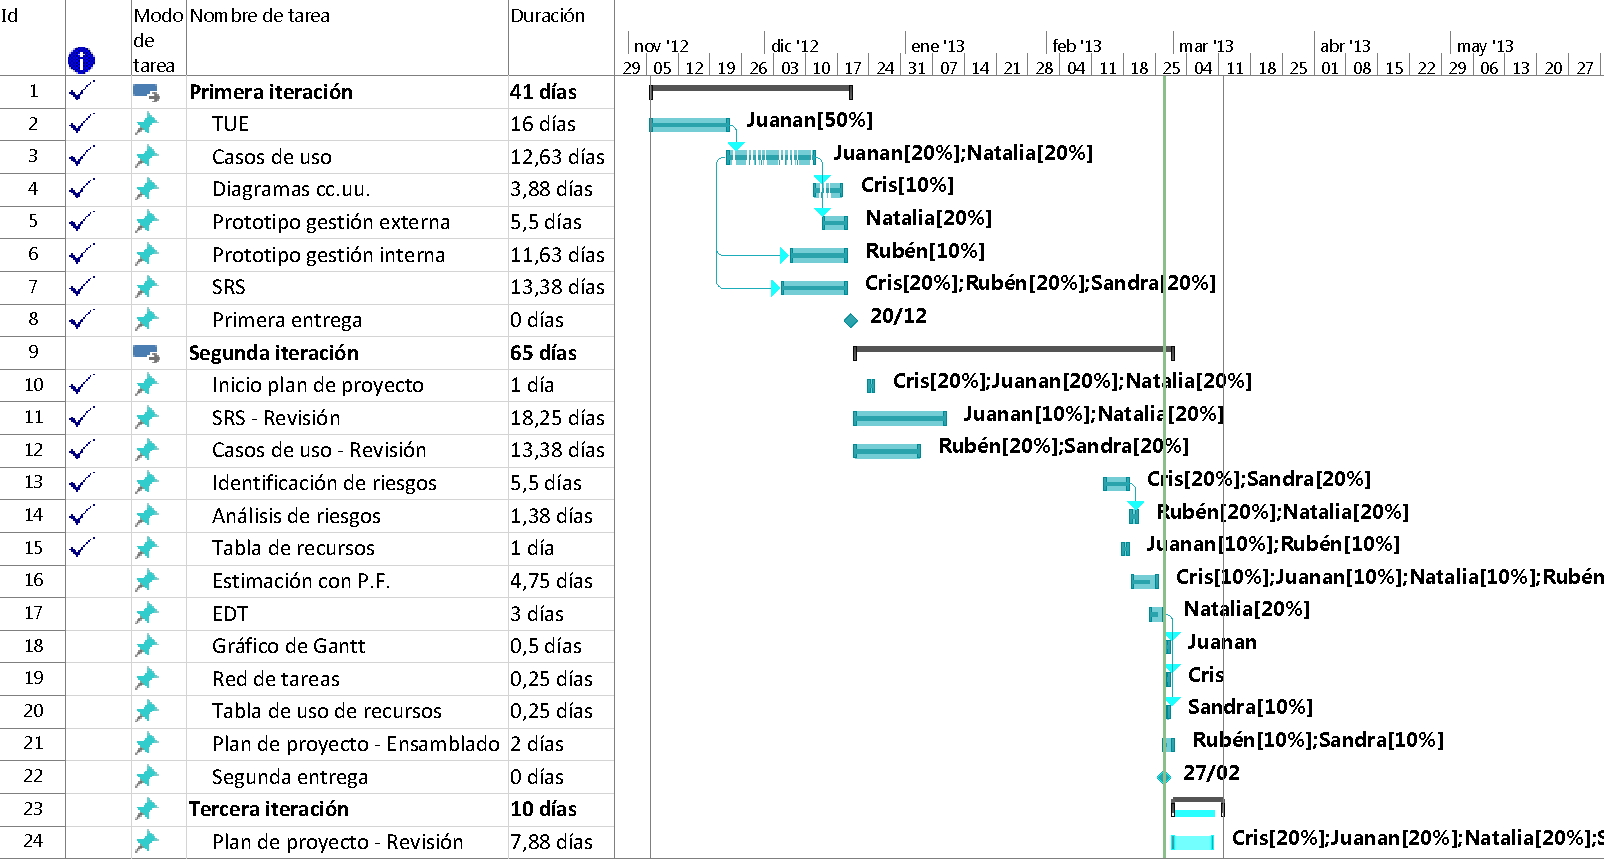
\includegraphics[scale=.8]{planific/Gantt.pdf}
			\end{figure}
		\end{landscape}

		\begin{landscape}
		\subsection{Red de tareas}
			\begin{figure}[h] \centering
			\vspace{1.1cm}
			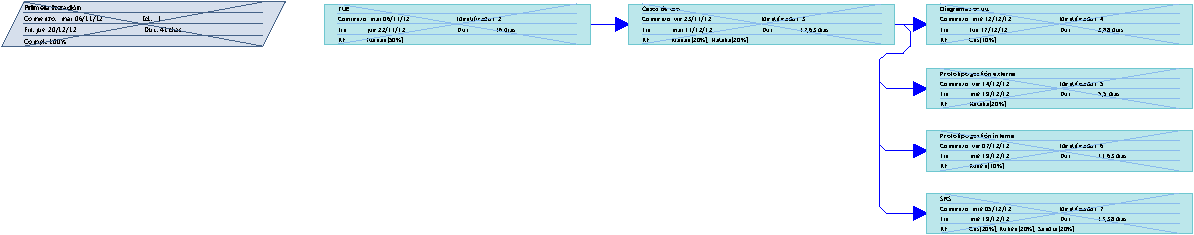
\includegraphics[scale=1]{planific/redtareas1.pdf}
			\caption{Red de tareas de la primera iteración}
			\end{figure}

			\begin{figure}[h] \centering
			\vspace{1.1cm}
			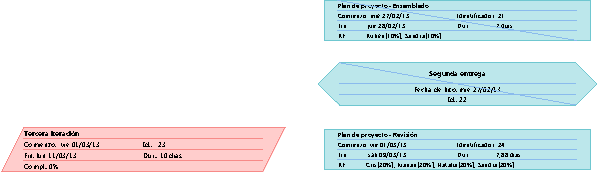
\includegraphics[scale=1.2]{planific/redtareas3.pdf}
			\caption{Red de tareas de la tercera iteración}
			\end{figure}

			\begin{figure}[h] \centering
			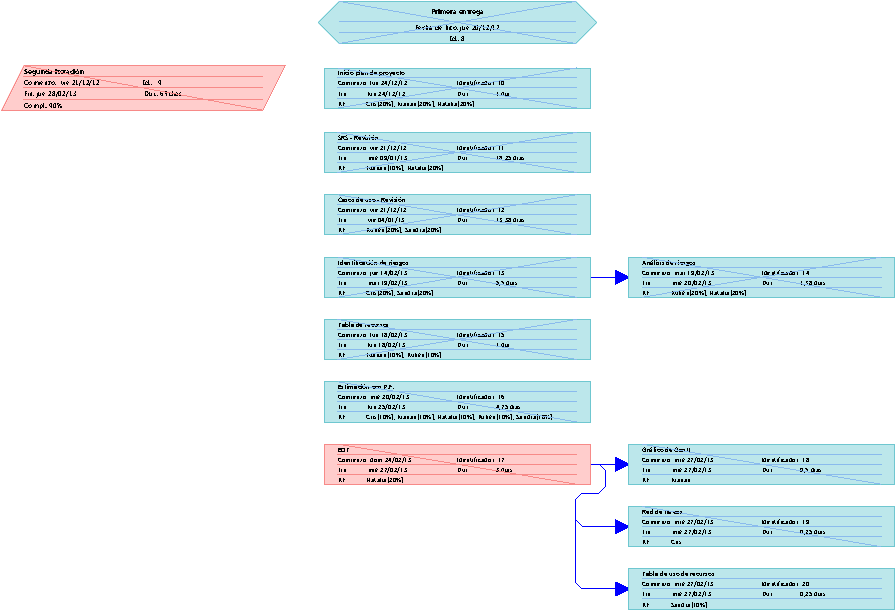
\includegraphics[scale=1.45]{planific/redtareas2.pdf}
			\caption{Red de tareas de la segunda iteración}
			\end{figure}
		\end{landscape}

		\subsection{Tabla de uso de recursos} %tabla?
	\section{Recursos del proyecto}
		\subsection{Personal}
			Para el equipo desarrollo de éste proyecto disponemos de una plantilla de dimensión reducida pero a su vez un equipo motivado por lo pensamos que la organización Descentralizado Democrático (DD) de Mantei puede resultar productiva. Esta organización se caracteriza por no tener un jefe permanente si no que se nombran para cada tarea y las decisiones y soluciones a problemas se llevan a consenso del grupo. Se asignarán las tareas de forma individual o por equipos bien definidos.

		\subsection{Hardware y software}
			El equipo de desarrollo cuenta, para la realización de sus tareas, con sus computadoras personales, además del uso de los laboratorios y las instalaciones de la Facultad de Informática y la Facultad de Matemáticas de la Universidad Complutense de Madrid, donde desarrollan su actividad académica.\\

			El \software utilizado consiste principalmente en herramientas para la elaboración de la documentación, y en las herramientas CASE para desarrollar las actividades de la Ingeniería del Software. En la fase de desarrollo y creación de prototipos se han utilizado compiladores y herramientas de desarrollo estándar. Citamos además la documentación empleada.

		\subsection{Lista de recursos}
			% Airline Common Environment (ACE)
% Proyecto de Ingeniería del Software
% Grupo Diedral 2013

% Plan de proyecto - Lista de recursos

\begin{itemize}
	\item Personal \\

		\recurso{1}	% id
		{Cristina Alonso Fernández}	% nombre
		{Miembro del equipo de desarrollo}	% descripción
		{}	% origen
		{Tiempo parcial}	% disponibilidad
		{}	% uso

		\recurso{2}
		{Natalia Angulo Herrera}
		{Miembro del equipo de desarrollo}
		{}
		{Tiempo parcial}
		{}

		\recurso{3}
		{Sandra Bermejo Cañadas}
		{Miembro del equipo de desarrollo}
		{}
		{Tiempo parcial}
		{}

		\recurso{4}
		{Juan Andrés Claramunt Pérez}
		{Miembro del equipo de desarrollo}
		{}
		{Tiempo parcial}
		{}

		\recurso{5}
		{Rubén Rafael Rubio Cuéllar}
		{Miembro del equipo de desarrollo}
		{}
		{Tiempo parcial}
		{}

	\item Componentes de software reutilizables \\

		\recurso{6}
		{Biblioteca gráfica \textit{Qt} 4.8 GPL}
		{Biblioteca para interfaces gráficas multiplataforma para C++. Disponible para otros lenguajes de programación.}
		{\textit{Digia} (anteriormente \textit{Nokia}). Licencia \textit{GPL}.}
		{Simultánea e ilimitada.}
		{Codificación y/o prototipado.}


		\recurso{6.5}
		{Iconos \textit{Tango}.}
		{Iconos para uso general dentro de una aplicación.}
		{\textit{Tango Desktop Project} (más detalles en \url{http://tango.freedesktop.org/}).}
		{Simultáneo e ilimitada.}
		{Codificación y/o prototipado.}

	\item Entorno de desarrollo: elaboración  de la documentación \\

		\recurso{7}
		{Sistema tipográfico {\rmfamily \TeX{}} y {\rmfamily\LaTeX{}}}
		{Distribuciones {\rmfamily\TeX{} Live} y {\rmfamily Mik\TeX{}}.}
		{Proyecto {\rmfamily\LaTeX{}3}. Licencia \textit{LPPL}.}
		{Simultánea y no limitada.}
		{Elaboración de la documentación durante todo el proyecto.}

		\recurso{8}
		{Paquetes {\rmfamily\LaTeX{}} de terceros}
		{Los paquetes {\rmfamily color}, {\rmfamily babel}, {\rmfamily xkeyval}, {\rmfamily ifthen}, {\rmfamily ifpdf}, {\rmfamily environ}, {\rmfamily amsmath},  {\rmfamily tabularx}, {\rmfamily supertabular}, {\rmfamily multirow}, {\rmfamily fancyhdr}, {\rmfamily tikz}, {\rmfamily hyphenat}, {\rmfamily anysize}, {\rmfamily graphicsx}, {\rmfamily float}, {\rmfamily rotating}, {\rmfamily hyperref}, {\rmfamily titletoc}, {\rmfamily glossaries} y {\rmfamily todonotes}.}
		{Autores y más información en \url{www.ctan.org}.}
		{Disponible en los equipos personales de los desarrolladores. Algunos miembros del equipo no cuentan con la distribución correctamente configurada. No disponible en los laboratorios de las facultades, salvo configuración \textit{ad hoc}.}
		{Elaboración de la documentación durante todo el proyecto.}

		\recurso{9}
		{Paquete {\rmfamily isdiedral}}
		{Paquete de {\rmfamily \LaTeX{}} elaborado para facilitar la generación de documentación durante el proyecto.}
		{Elaboración propia.}
		{Simultánea y no limitada.}
		{Elaboración de la documentación durante todo el proyecto.}

		\recurso{10}
		{Clases de terceros para {\rmfamily \LaTeX{}}}
		{Las clases {\rmfamily ltxdoc} y {\rmfamily beamer}, para elaboración de documentación de paquetes y de presentaciones de diapositivas respectivamente.}
		{Autores y más información en \url{www.ctan.org}.}
		{Simultánea y no limitada.}
		{Elaboración de la documentación durante todo el proyecto.}

		\recurso{11}
		{Familia de fuentes {\rmfamily Latin Modern}}
		{Familia de fuentes serifadas derivada de {\rmfamily Computer Modern}, familia tipográfica por defecto de {\rmfamily \TeX{}}.}
		{Mantenido por Bogusław Jackowski y Janusz M. Nowacki.}
		{Simultánea y no limitada.}
		{Elaboración de la documentación durante todo el proyecto.}

		\recurso{12}
		{\textit{ArgoUML}}
		{Herramienta de modelado UML.}
		{Licencia \textit{EPL} 1.0. Página oficial: \url{http://argouml.tigris.org}.}
		{Simultánea e ilimitada. Ejecutable en los laboratorios de la Facultad de Informática.}
		{Elaboración de los diagramas de casos de uso y clases en el diseño.}


	\item Entorno de desarrollo: herramientas para la comunicación \\
		
		\recurso{13}
		{\textit{RiouxSVN}}
		{Repositorio de control de versiones basado en \textit{Subversion}.}
		{Ver \url{http://riouxsvn.com}.}
		{Continua y simultánea. Cortes de servicio puntuales por labores de mantenimiento.}
		{Gestión de la configuración, durante todo el proyecto.}

		\recurso{14}
		{\textit{Assembla}}
		{Repositorio de control de versiones basado en \textit{Subversion} como copia de respaldo del
		repositorio corriente.}
		{Ver \url{http://www.assembla.com}.}
		{Continua y simultánea.}
		{Gestión de la configuración, durante todo el proyecto.}

		\recurso{15}
		{Correo electrónico de la Universidad Complutense de Madrid}
		{Correo institucional de la universidad.}
		{}
		{Continua y simultánea.}
		{Comunicación del equipo de desarrollo.}

		\recurso{16}
		{\textit{Google Drive}}
		{Sistema de almacenamiento de documentos. Accedido a través de las \textit{Google Apps} de la Universidad Complutense de Madrid.}
		{}
		{Continua y simultánea.}
		{Comunicación del equipo de desarrollo.}

	\item Entorno de desarrollo: herramientas CASE \\

		\recurso{17}
		{\textit{Microsoft Project}}
		{Programa de administración de proyectos.}
		{\textit{Microsoft Corportation}, a través del programa \textit{DreamSpark} asociado a la Facultad de Informática de la UCM.}
		{Continua y simultánea.}
		{Planificación y gestión del proyecto.}

	\item Entorno de desarrollo: equipo físico \\

		\recurso{17}
		{Uso de los laboratorios}
		{Uso de los laboratorios de la \textit{Facultad de Informática} y la \textit{Facultad de Ciencias Matemáticas} de la UCM.}
		{}
		{Restringida al horario y disponibilidad de plazas.}
		{Durante todo el proyecto.}

		\recurso{18}
		{Ordenadores personales de los miembros del equipo de desarrollo}
		{Ordenadores personales para trabajo por separado.}
		{}
		{No determinada.}
		{Durante todo el proyecto.}

		\recurso{19}
		{Equipo utilizado en las exposiciones}
		{Proyector, pizarra, ordenador del profesor\ldots}
		{}
		{Cuando corresponde.}
		{En las exposiciones públicas en clase.}

	
	\item Entorno de desarrollo: programación de prototipos y versiones del producto \\
		
		\recurso{20}
		{Colección de Compiladores de GNU (GCC)}
		{Colección de compiladores multiplataforma. Especialmente usados los de C y C++.}
		{\textit{Free Software Fundation}. Licencia \textit{GPL}.}
		{Simultánea y no limitada.}
		{Elaboración de prototipos y/o versión final.}

		\recurso{21}
		{Compilador de \textit{Microsoft Visual C++} v11}
		{Compilador de C++ para \textit{Windows}.}
		{\textit{Microsoft Corporation}.}
		{Simultánea y no limitada.}
		{Elaboración de prototipos y/o versión final.}

		\recurso{22}
		{Java}
		{Máquina virtual y entorno de desarrollo de Java, por ejemplo \textit{OpenJDK} 7.}
		{\textit{Oracle Corporation}.}
		{Simultánea y no limitada.}
		{Elaboración de prototipos y/o versión final. Elaboración de herramientas.}

		
	\item Entorno de desarrollo: material de referencia

		\recurso{23}
		{Libro \textit{Ingeniería del Software: un enfoque práctico}}
		{El libro \cite{PSMAN}.}
		{Roger S. Pressman}
		{Sujeta a la disponibilidad de ejemplares en la biblioteca de la facultad.}
		{Todo el proyecto.}

		\recurso{24}
		{Estándares de Ingeniería de Software}
		{Estándares accesibles a través de \textit{IEEEXplore\marcaregistrada} mediante la cuenta de la Universidad Complutense de Madrid.}
		{IEEE.}
		{Simultánea e ilimitada al conjunto de estándares necesarios.}
		{Todo el proyecto.}

		\recurso{25}
		{Documentación de C++}
		{Documentación de C++ disponible en los sitios web \url{www.cplusplus.com} y \url{http://es.cppreference.com/}. Estándares disponibles en \url{www.open-std.com} y el libro \emph{El lenguaje de programación C++} de Bjarne Stroustrup \cite{STROUSTRUP}.}
		{Sus correspondientes autores.}
		{Simultánea y no limitada. Para el libro, sujeta a la disponibilidad de ejemplares en la biblioteca aunque disponible
		en inglés de forma ilimitada y simultánea por medio de la biblioteca de la universidad.}
		{Codificación y/o prototipado.}

		\recurso{26}
		{Documentación de Java}
		{Documentación de la API de Java disponible en \url{http://docs.oracle.com/javase/7/docs/api/} y los apuntes de la asignatura \textit{Tecnología de la Programación} \cite{AP_TP}.}
		{Sus correspondientes autores.}
		{Simultánea y no limitada.}
		{Codificación y/o prototipado.}
\end{itemize}


	\section{Organización del personal}
		\subsection{Estructura de equipo}
		El escaso número de miembros del que consta el equipo de trabajo ha dificultado el establecimiento de una estructura compleja del mismo, sin embargo, sí se han realizado unas pequeñas divisiones para facilitar y organizar de manera más clara el trabajo. En este sentido, Rubén ha sido el coordinador del equipo durante todo el desarrollo del proyecto, debido a sus mayores conocimientos en las herramientas que podían utilizarse. \\
		El resto del equipo, siguiendo las pautas del coordinador, ha realizado un trabajo similar, bien repartiendo las partes del proyecto entre todos los miembros del mismo y realizando rotaciones, o bien dividiendo el trabajo a realizar en subgrupos de dos personas, revisando posteriormente el trabajo del resto de los miembros del equipo. En ambos casos, se ha intentado garantizar la homogeneidad y el trabajo de todos los miembros en todos los aspectos del proyecto.
		\subsection{Informes de gestión}
		Las comunicaciones entre los miembros del equipo de desarrollo se realizan principalmente a través del correo electrónico de la Universidad Complutense de Madrid. Mediante este correo nos informamos acerca de la organización del trabajo, establecemos las pautas a seguir, fijamos las próximas reuniones del equipo\ldots También nos sirve para consultar o comunicar cualquier duda, sugerencia o problema encontrado durante la realización del trabajo. \\
		Cuando un miembro del equipo genera	nueva documentación, la deposita en el repositorio \textit{Assembla} (hasta febrero de 2013 en \textit{RiouxSVN}), añadiendo un comentario con las principales modificaciones, informando así al resto del equipo. Todos los documentos solicitados por el cliente en las distintas entregas, así como el material empleado en las exposiciones y la documentación interna es compartido por el equipo de desarrollo y por el cliente a través de \textit{Google Drive}.
	\section{Mecanismo de seguimiento y control}
		\subsection{Garantía de calidad y control}
		El objetivo de la garantía de calidad es proporcionar la gestión para informar de los datos necesarios sobre la calidad del producto. Para garantizar la calidad se aplicaran actividades de protección y control de calidad. Mediante procesos de verificación y validación determinaremos si los productos desarrollados se ajustan a los requisitos. Estos procesos se verán materializados en evaluaciones, auditorías, inspecciones y revisiones periódicas, pruebas del software, estándares que se pueden aplicar al proyecto, procedimientos para información y seguimiento de errores, y documentos producidos.
		\subsection{Gestión y control de cambios}
			Se consideran los siguientes elementos de control: el desarrollo de casos de uso denotado \textit{CCUU}, los diagramas de casos de uso denotados \textit{Diagramas CCUU}, el documento de especificación de requisitos \software denotado \textit{SRS}, el plan de proyecto, el prototipo de gestión externa y el prototipo de gestión interna.\\

			La notación de la versión del \software utiliza al menos dos dígitos numéricos, siendo el más representativo el situado más a la izquierda. Este número representa el número de entregas terminadas, de forma que la versión entregada en la primera entrega es la 1.0, la entregada en segundo término es la 2.0 y así sucesivamente. Versiones intermedias serán representadas mediante la numeración menos significativa. Cuando pueda resultar útil se indicará la revisión del sistema de control de versiones después del número de versión como en \verb|1.0-rv50|. La notación de versión de los elementos será independiente de la versión general.
		
		\begin{itemize}
			\item[\bfseries 0.1] $\{$CCUU 0.1, Diagramas CCUU 0.1$\}$
			\item[\bfseries 0.2] $\{$CCUU 0.2, Diagramas CCUU 0.1, SRS 0.2, Prototipo Interna 0.1, Prototipo Externa 0.1$\}$
			\item[\bfseries 0.3] $\{$CCUU 0.3, Diagramas CCUU 0.3, SRS 0.3, Prototipo Interna 0.2, Prototipo Externa 0.2$\}$
			\item[\bfseries 1.0] $\{$CCUU 1.0, Diagramas CCUU 1.0, SRS 1.0, Prototipo Interna 1.0, Prototipo Externa 1.0$\}$ de los Casos de Uso 1.1$\}$
			\item[\bfseries 2.0] $\{$CCUU 2.0, Diagramas CCUU 1.0, SRS 2.0, Plan de Proyecto 2.0 (EDT 2.0, Riesgos 2.0, Estimación 2.0, Planificación 2.0) $\}$
		\end{itemize}
		
	\newpage
	\section{Apéndices}
		\appendix
		\subsection{Actividad del repositorio}
			\tiny

% Usa como impresor de fechas el del paquete "isdiedral"
% Otra opción es "isodate" (pero no soporta español aún)
\let \printdate = \imprimefecha

% Comando de uso particular para imprimir revisiones
\newcommand*{\reporev}[3]{\item #1 (#2, \printdate{#3}).}

\begin{multicols}{2}
\begin{enumerate}
	\renewcommand*{\theenumi}{\bfseries r\arabic{enumi}}

	\reporev{Creación de la estructura general del repositorio}{Automático}{22.11.2012}
	\reporev{Primera subida de archivos}{NAH}{22.11.2012}
	\reporev{Añadido diagrama de gestión interna y documentación del paquete isdiedral}{RRC}{24.11.2012}
	\reporev{Añadidos 3 casos de uso del primer reparto}{NAH}{24.11.2012}
	\reporev{Borrador de 2 casos de uso. Inclusión de los casos de uso en el documento}{RRC}{25.11.2012}
	\reporev{Subidos casos de uso: crear nómina y programar revisión, y actualizado fichero casosdeuso}{JCP}{25.11.2012}
	\reporev{Dos casos de uso Gestión Externa (presentar reclamaciones y realizar pago billetes)}{NAH}{28.11.2012}
	\reporev{Solución temporal a las tablas multipágina}{RRC}{28.11.2012}
	\reporev{Cambios técnicos: separación de secuencias, índice y desactivación de separación de palabras al final de línea}{RRC}{2.12.2012}
	\reporev{Nuevo caso de uso: consulta vuelos}{RRC}{2.12.2012} % r10
	\reporev{Más casos de uso}{SBC}{7.12.2012}
	\reporev{Proto-prototipo del sistema de gestión interna}{RRC}{10.12.2012}
	\reporev{Casos de uso: comprar billete y mostrar ofertas de GE; consultar nómina y consultar plan de vuelo de GI}{CAF}{10.12.2012}
	\reporev{Subida tabla ver info vuelo}{JCP}{10.12.2012}
	\reporev{Modificados casos de uso: consultar inventario, modificar items inventario, consultar plan de vuelo y entrada material}{NAH}{11.12.2012}
	\reporev{Modificados casos de uso que hice y he vuelto a subir los diagramas de gestión interna pues no los había subido correctamente}{NAH}{12.12.2012}
	\reporev{Nuevos casos de uso de gestión externa}{NAH}{12.12.2012}
	\reporev{Vuelvo a subir el diagrama gestión interna añadido un caso de uso que se nos había olvidado (crear nómina). Hecho el diagrama de gestión externa. Dividido el caso de uso de realizar pago en tres partes}{NAH}{12.12.2012}
	\reporev{Corregidos errores LaTeX en casos de uso. Esquema de SRS. Esquema de diagramas en LaTeX}{RRC}{12.12.2012}
	\reporev{Cambios en el prototipo GI. Prototipo GE}{RRC}{12.12.2012} % r20
	\reporev{Orden alfabético en casos de uso. Arreglados errores}{RRC}{12.12.2012}
	\reporev{Casos de uso (comprar billete, mostrar ofertas, consultar nómina y consultar plan de vuelo) modificados}{CAF}{12.12.2012}
	\reporev{Modificado el diagrama añadiendo el nuevo caso de uso consultar ficha empleado. Incluido en fichero casos de uso}{NAH}{13.12.2012}
	\reporev{Corregido error de sintaxis en consultar plan de vuelo}{NAH}{13.12.2012}
	\reporev{Modificacion casos de uso: accederGE, accederGI, registrarse y ModificarItemsInventario}{SBC}{13.12.2012}
	\reporev{{}[QPrototipo] Añadida pantalla de inicio}{RRC}{13.12.2012}
	\reporev{Cambios en laboratorio. Comienzo de SRS}{todos [NAH]}{13.12.2012}
	\reporev{Revisión de casos de uso, pequeños cambios}{JCP}{14.12.2012}
	\reporev{Revisados y añadidos casos de uso. Algo de las Srs}{RRC}{14.12.2012}
	\reporev{{}[SRS] Añadido soporte para bibliografía con BibTex, añadido srsfuncion (comando de sección de nivel 4), control de versiones e intento de espeficación. [Casos de uso] Algún cambio}{RRC}{15.12.2012}
	\reporev{{}[Casos de uso] Revisión de los que me correspondían (bastantes cambios)}{RRC}{15.12.2012} % r30
	\reporev{Nuevos casos de uso: dar de baja cliente y configurar sistema general}{NAH}{15.12.2012}
	\reporev{Revisados casos de uso: comprarBillete, consultarInventario, consultarFichaEmpleado, configurarNomina; y añadidos:\break introducirPlanDeVuelo, efectuarEmbarque}{SBC}{15.12.2012}
	\reporev{Casos de uso revisados: editarInformacionEconomica,\break IniciarPagoBilletesDeVuelo, ModificarItemsInventario, programarHorarios, realizarPagoconTarjeta, registrarEmpleado, verificarRegistroEmpleado. He eliminado pago con PayPal pues no es frecuente en compra de billetes de vuelo}{CAF}{15.12.2012}
	\reporev{Cambio de nombres [erróneo]}{CAF}{15.12.2012}
	\reporev{Revisiones y añadidos dos casos de uso}{JCP}{15.12.2012}
	\reporev{Renombrados ya que causaban conflicto [ver r35]}{JCP}{15.12.2012}
	\reporev{{}[SRS] Modificada la función Ver plan de vuelo y completados otros epígrafes}{RRC}{13.12.2012}
	\reporev{{}[SRS] funciones del producto}{JCP}{15.12.2012}
	\reporev{SRS de mis casos de uso (llevan el nombre del caso de uso al que corresponden con un SRS delante).}{CAF}{16.12.2012} % r40
	\reporev{{}[SRS] añadido editar cliente en funciones de gestión interna, añadida sección atributos del sistema de software y completada sección alcance}{JCP}{16.12.2012}
	\reporev{{}[SRS] añadidos: consultar nómina, acceder gestión externa, editar empleado, acceder horarios, presentar reclamaciones, consultar vuelos}{JCP}{16.12.2012}
	\reporev{He añadido las funciones de los SRS. Además he modificado también con los campos que me tocaban realizar la SRS (documento general). También he subido los casos de uso revisados}{NAH}{14.12.2012}
	\reporev{{}[SRS] Unidas las diferentes modificaciones manualmente (si alguien nota que falta algo...). Extraídas todas las funciones del archivo principal. Hay 2 iniciar sesión interno y ninguno externo. El significado de registrar entrada material no es adecuado}{RRC}{16.12.2012}
	\reporev{Renombrado un archivo}{NAH}{16.12.2012}
	\reporev{Cambios derivados del renombramiento anterior en el documento general}{NAH}{16.12.2012}
	\reporev{Eliminado el caso de uso pago con PayPal}{NAH}{16.12.2012}
	\reporev{Cambios en registrar entradas de material}{NAH}{16.12.2012}
	\reporev{Diagramas de casos de uso con argoUML}{todos (NAH)}{16.12.2012}
	\reporev{Revisión de las SRS e inclusiones en el glosario}{NAH}{16.12.2012} % r50
	\reporev{Introducido el generador de plantillas para pantallas}{RRC}{16.12.2012}
	\reporev{{}[Prototipo Interno] Añadidas viejas pantallas olvidadas, ultraesqueleto de FListado y recursos (iconos Tango)}{RRC}{16.12.2012}
	\reporev{Modifico la parte de configurar sistema en los srs.tex y el glosario por algunas modificaciones realizadas ahí}{NAH}{16.12.2012}
	\reporev{Modificación del commit anterior [r52]}{NAH}{16.12.2012}
	\reporev{Movidas las pantallas a la carpeta pantallas. Ahora el prototipo NO compila temporalente}{RRC}{16.12.2012}
	\reporev{Cambiado ref por nameref. Líos varios}{RRC}{16.12.2012}
	\reporev{Pantallas: dar de baja cliente, programar revisión y registrar entrada material; glosario y SRS; casos de uso: mostrar ofertas, programar oferta y acceder a una oferta (SRS y diagramas)}{NAH}{17.12.2012}
	\reporev{+1 pantallas Programaroferta subida}{NAH}{17.12.2012}
	\reporev{Pantalla Editar Empleado}{JAP}{17.12.2012}
	\reporev{Pantallas casos de uso de Gestión Interna (modificarItemsInventario, registrarEmpleado, verificarRegistroEmpleado, programarHorarios y editarInformacionEconomica)}{CAF}{17.12.2012} % r60
	\reporev{Pequeñas modificaciones}{CAF}{17.12.2012}
	\reporev{Pequeñas modificaciones en SRS de casos uso}{CAF}{17.12.2012}
	\reporev{Pantalla ConsultaNomina}{JAP}{17.12.2012}
	\reporev{Modificaciones en los casos de uso}{CAF}{17.12.2012}
	\reporev{Añadidas pantallas: consultar inventario, consultar ficha empleado, dar de baja empleado, configurar nómina, introducir plan de vuelo y efectuar embarque}{SBC}{17.12.2012}
	\reporev{Añado también el formato imagen de las pantallas}{SBC}{17.12.2012}
	\reporev{Especificación de requisitos de mis casos de uso}{SBC}{17.12.2012}
	\reporev{Implementación básica del prototipo. Ya no subáis más pantallas}{RRC}{18.12.2012}
	\reporev{Añadidas algunas imágenes al documento srs}{NAH}{18.12.2012}
	\reporev{Prototipo web}{NAH}{18.12.2012} % r70
	\reporev{Arreglados errores en las SRS}{RRC}{18.12.2012}
	\reporev{Añadida presentación-exposición}{RRC}{18.12.2012}
	\reporev{Mejoradas (o no) algunas pantallas del prototipo}{RRC}{18.12.2012}
	\reporev{Quitado comentario ya modificado}{NAH}{19.12.2012}
	\reporev{Subo el prototipo web con todo más o menos hecho}{NAH}{19.12.2012}
	\reporev{Resubo Realizar pago final que se había colado una versión antigua}{NAH}{19.12.2012}
	\reporev{Subo el SRS compilado con todos los archivos que genera a petición de Juan Andrés}{NAH}{19.12.2012}
	\reporev{He añadido a la SRS: resumen, supuestos y dependencias, requisitos de rendimiento}{SBC}{19.12.2012}
	\reporev{Añadidos SRS finales}{CAF}{19.12.2012}
	\reporev{Eliminados archivos innecesarios y altamente conflictivos}{RRC}{19.12.2012} % r80
	\reporev{Mejorada considerablemente la apariencia de los diagramas de la presentación. Logo transparente}{RRC}{19.12.2012}
	\reporev{{}[Casos de uso] Diagramas añadidos al fichero casos de uso}{RRC}{19.12.2012}
	\reporev{Cambios en el prototipo web}{NAH}{19.12.2012}
	\reporev{Ligera modificación en la web (logo sin fondo) y tabla de vuelos de modificadas las terminales}{NAH}{19.12.2012}
	\reporev{Error al subirlo. Esta es la versión buena.}{NAH}{19.12.2012}
	\reporev{Eliminada copia de logotipo duplicada}{NAH}{19.12.2012}
	\reporev{Añadidas palabras al glosario}{NAH}{19.12.2012}
	\reporev{Pequeña correción}{JAP}{19.12.2012}
	\reporev{Añadida función perdida de procedencia desconocida}{RRC}{19.12.2012}
	\reporev{Cambios de estilo en el prototipo interno}{RRC}{19.12.2012} % r90
	\reporev{Otra subida del prototipo de gestión externa}{NAH}{19.12.2012}
	\reporev{Incluidos todos los casos de uso}{NAH}{20.12.2012}
	\reporev{Corregidos errores e incluidos casos de uso}{RRC}{20.12.2012}
	\reporev{Arreglados los conflictos con el commit de Natalia. Salen 35 casos de uso, antes salían 34. Latex dice que no hay repes}{RRC}{20.12.2012}
	\reporev{Actualizado el árbol de directorios para aislar los casos de uso}{RRC}{21.12.2012}
	\reporev{Modelo de plan de proyecto y tabla de descripción de riesgo}{RRC}{24.12.2012}
	\reporev{Subo los casos de uso revisados de Personal de Recursos Humanos y Directivos.}{NAH}{25.12.2012}
	\reporev{Ligeras modificaciones en casos de uso del Personal de planificación de operaciones y del Personal de atención al cliente}{SBC}{26.12.2012}
	\reporev{Completando el commit anterior.}{SBC}{26.12.2012}
	\reporev{Revisión de SRS: acceder, configurarNomina, consultarFichaEmpleado, consultarHorarios, consultarNomina, darDeBajaEmpleado,\break obtenerInfoEconomica, registrarEmpleado, verificarRegistroEmpleado. He añadido a cada SRS un nuevo item como hizo Rubén que indica la prioridad de la función}{NAH}{27.12.2012} % r100
	\reporev{Revisado en srs: Resumen, Características del usuario (modificado algo muy mínimo) y supuestos y dependencias (he añadido un párrafo)}{NAH}{27.12.2012}
	\reporev{Solucionados algunos errores en los documentos (ausencia de corchetes y presencia de comas)}{RRC}{28.12.2012}
	\reporev{{}[Prototipo] Muchos cambios, muchos más archivos, pocas mejoras}{RRC}{30.12.2012}
	\reporev{{}[Prototipo] Arreglados ciertos errores y algunas mejoras}{RRC}{31.12.2012}
	\reporev{Cambios en los apartados de las SRS que me tocaron. Ortografía. Añadidos metadatos PDF}{RRC}{03.1.2013}
	\reporev{Eliminado directorio `prototipo web dreamweaver' porque es copia de `prototipo\_externa'}{RRC}{3.1.2013}
	\reporev{Revisión de casos de uso y sus SRS correspondientes. Añadido caso de uso realizar mantenimiento y dividido el antiguo caso de uso efectuar embarque en: facturar y realizar embarque}{CAF}{4.1.2013}
	\reporev{Corregidos errores LaTeX. Cambios en los casos de uso. Nuevo caso de uso `incidencias sistema'}{RRC}{4.1.2013}
	\reporev{Realizar mantenimiento actualizado, sin que redirija a Modificar inventario}{CAF}{4.1.2013}
	\reporev{Añadidas funciones Realizar mantenimiento y Facturar, así como pequeños cambios en SRS: Perspectiva del producto, Supuestos y dependencias}{CAF}{4.1.2013} % r110
	\reporev{{}[Prototipo] Corregidos algunos graves errores y añadida cierta funcionalidad aparente con persistencia}{RRC}{6.1.2013}
	\reporev{Cambios en la SRS y el plan de proyecto}{RRC}{10.1.2013}
	\reporev{Cambios en los documentos para incluir encabezados}{RRC}{10.1.2013}
	\reporev{Añadido un cuadro de riesgo (Pr) y especificación del formato de fecha (SRS)}{RRC}{23.1.2013}
	\reporev{Reorganización de archivos y portadas}{RRC}{16.2.2013}
	\reporev{Índice de funciones en SRS y otros cambios}{RRC}{16.2.2013}
	\reporev{Añadida estructura del programa de gestión interna}{RRC}{18.2.2013}
	\reporev{Subido riesgo Inactividad por periodo examenes. Duda en la parte de autor/departamento que realiza el riesgo}{NAH}{19.2.2013}
	\reporev{Repito lo anterior, que no se ha subido.}{NAH}{19.2.2013}
	\reporev{Un nuevo riesgo: softwarenoreutilizable}{NAH}{19.2.2013} % r120
	\reporev{Corregidos algunos fallos}{NAH}{19.2.2013} % r120	
	\reporev{Última tabla de riesgo: faltacomunicacioncliente. Comentamos algunas dudas mañana}{NAH}{19.2.2013}
	\reporev{Cambio mínimo de acuerdo a la correción}{RRC}{19.2.2013}
	\reporev{planproyecto modificado. Hay cosas que hay que revisar mañana}{NAH}{20.2.2013}
	\reporev{3 riesgos añadidos. Cambios en obsolescencia de tecnologias utilizadas en: - Impacto de N a M - Probabilidad de M a B}{CAF}{20.2.2013}
	\reporev{Plan de proyecto actualizado}{CAF}{20.2.2013}
	\reporev{Subidos otros 3 riesgos y añadidos en planproyecto}{SBC}{20.2.2013}
	\reporev{Riesgos}{JCP}{20.2.2013}
	\reporev{Corregidos errores de sintaxis. Abreviados nombres de archivo. Anexo de control de versiones. Añadida plantilla para la presentación}{RRC}{20.2.2013}
	\reporev{Algunos cambios por correciones}{RRC}{21.2.2013} % r130
	\reporev{Tabla de enumeración de riesgos. Algunos cambios más}{RRC}{21.2.2013} 
	\reporev{Cambiada la tabla de descripción de riesgos}{RRC}{21.2.2013}
	\reporev{Modificaciones en hoja de riesgos}{RRC}{21.2.2013}
	\reporev{Nuevos riesgos}{RRC}{21.2.2013}
	\reporev{Riesgo añadido: ensamblar}{JCP}{21.2.2013}
	\reporev{Lista de materiales y otros cambios}{RRC}{21.2.2013}
	\reporev{Pequeñas modificaciones en riesgos y añadido nuevo riesgo desconocimientotecnologias}{CAF}{22.2.2013}
	\reporev{Plan de proyecto. Añadidas declaración y funciones principales en Ámbito y estructura del equipo en Organización personal}{CAF}{22.2.2013}
	\reporev{Añadidos archivos de Cocomo y Project}{RRC}{22.2.2013}
	\reporev{id riesgos modificados}{NAH}{22.2.2013} % r140
	\item[$\star$] {\itshape Actualizado a 23 de febrero de 2013}


\end{enumerate}
\end{multicols}

\normalsize

% fin

		
		\newpage
		\normalsize
		\nocite{PSMAN}
		\bibliography{planproyecto}
		\bibliographystyle{apalike}
\end{document}
